%%%%%%%%%%%%%%%%%%%%%%%%%%%%%%%%%%%%%%%%%
% Classicthesis Typographic Thesis
% LaTeX Template
% Version 1.3 (15/2/14)
%
% This template has been downloaded from:
% http://www.LaTeXTemplates.com
%
% Original author:
% André Miede (http://www.miede.de)
%
% License:
% CC BY-NC-SA 3.0 (http://creativecommons.org/licenses/by-nc-sa/3.0/)
%
% General Tips:
% 1) Make sure to edit the classicthesis-config.file
% 2) New enumeration (A., B., C., etc in small caps): \begin{aenumerate} \end{aenumerate}
% 3) For margin notes: \marginpar or \graffito{}
% 4) Do not use bold fonts in this style, it is designed around them
% 5) Use tables as in the examples
% 6) See classicthesis-preamble.sty for useful commands
%
%%%%%%%%%%%%%%%%%%%%%%%%%%%%%%%%%%%%%%%%%

%----------------------------------------------------------------------------------------
%	PACKAGES AND OTHER DOCUMENT CONFIGURATIONS
%----------------------------------------------------------------------------------------

\documentclass[
		twoside,openright,titlepage,numbers=noenddot,headinclude,%1headlines,
                footinclude=true,cleardoublepage=empty,
                BCOR=5mm,paper=a4,fontsize=11pt, % Binding correction, paper type and font size
                ngerman,american, % Languages
                ]{scrreprt} 
                
% Includes the file which contains all the document configurations and packages - make sure to edit this file
%%%%%%%%%%%%%%%%%%%%%%%%%%%%%%%%%%%%%%%%%
% Thesis Configuration File
%
% The main lines to change in this file are in the DOCUMENT VARIABLES
% section, the rest of the file is for advanced configuration.
%
%%%%%%%%%%%%%%%%%%%%%%%%%%%%%%%%%%%%%%%%%

%----------------------------------------------------------------------------------------
%	DOCUMENT VARIABLES
%	Fill in the lines below to enter your information into the thesis template
%	Each of the commands can be cited anywhere in the thesis
%----------------------------------------------------------------------------------------

% Remove drafting to get rid of the '[ Date - classicthesis version 4.0 ]' text at the bottom of every page
\PassOptionsToPackage{eulerchapternumbers,listings,drafting, pdfspacing, subfig,beramono,parts}{classicthesis}
% Available options: drafting parts nochapters linedheaders eulerchapternumbers beramono eulermath pdfspacing minionprospacing tocaligned dottedtoc manychapters listings floatperchapter subfig
% Adding 'dottedtoc' will make page numbers in the table of contents flushed right with dots leading to them

\newcommand{\myTitle}{A new approach to Economic Geography}
\newcommand{\mySubtitle}{An Homage to The Elements of Typographic Style\xspace}
\newcommand{\myDegree}{Docteur en Physique Th\'eorique\xspace}
\newcommand{\myName}{R\'emi Louf\xspace}
\newcommand{\myProf}{Marc Barthelemy\xspace}
\newcommand{\myOtherProf}{Put name here\xspace}
\newcommand{\mySupervisor}{Put name here\xspace}
\newcommand{\myFaculty}{Put data here\xspace}
\newcommand{\myDepartment}{Put data here\xspace}
\newcommand{\myUni}{Université Pierre et Marie Curie\xspace}
\newcommand{\myLocation}{Darmstadt\xspace}
\newcommand{\myTime}{June 2015\xspace}
\newcommand{\myVersion}{version 1.0\xspace}

%----------------------------------------------------------------------------------------
%	USEFUL COMMANDS
%----------------------------------------------------------------------------------------

\newcommand{\ie}{i.\,e.}
\newcommand{\Ie}{I.\,e.}
\newcommand{\eg}{e.\,g.}
\newcommand{\Eg}{E.\,g.} 

\newcounter{dummy} % Necessary for correct hyperlinks (to index, bib, etc.)
\providecommand{\mLyX}{L\kern-.1667em\lower.25em\hbox{Y}\kern-.125emX\@}

%----------------------------------------------------------------------------------------
%	PACKAGES
%----------------------------------------------------------------------------------------

\usepackage{lipsum} % Used for inserting dummy 'Lorem ipsum' text into the template

%------------------------------------------------
 
\PassOptionsToPackage{latin9}{inputenc} % latin9 (ISO-8859-9) = latin1+"Euro sign"
\usepackage{inputenc}
 
 %------------------------------------------------

%\PassOptionsToPackage{ngerman,american}{babel}  % Change this to your language(s)
% Spanish languages need extra options in order to work with this template
%\PassOptionsToPackage{spanish,es-lcroman}{babel}
\usepackage{babel}

%------------------------------------------------			

\PassOptionsToPackage{square,numbers}{natbib}
 \usepackage{natbib}
 
 %------------------------------------------------

\PassOptionsToPackage{fleqn}{amsmath} % Math environments and more by the AMS 
 \usepackage{amsmath}
 
 %------------------------------------------------

\PassOptionsToPackage{T1}{fontenc} % T2A for cyrillics
\usepackage{fontenc}

%------------------------------------------------

\usepackage{xspace} % To get the spacing after macros right

%------------------------------------------------

\usepackage{mparhack} % To get marginpar right

%------------------------------------------------

\usepackage{fixltx2e} % Fixes some LaTeX stuff 

%------------------------------------------------

\PassOptionsToPackage{smaller}{acronym} % Include printonlyused in the first bracket to only show acronyms used in the text
\usepackage{acronym} % nice macros for handling all acronyms in the thesis

%------------------------------------------------

%\renewcommand*{\acsfont}[1]{\textssc{#1}} % For MinionPro
\renewcommand{\bflabel}[1]{{#1}\hfill} % Fix the list of acronyms

%------------------------------------------------

\PassOptionsToPackage{pdftex}{graphicx}
\usepackage{graphicx} 

%----------------------------------------------------------------------------------------
%	FLOATS: TABLES, FIGURES AND CAPTIONS SETUP
%----------------------------------------------------------------------------------------

\usepackage{tabularx} % Better tables
\setlength{\extrarowheight}{3pt} % Increase table row height
\newcommand{\tableheadline}[1]{\multicolumn{1}{c}{\spacedlowsmallcaps{#1}}}
\newcommand{\myfloatalign}{\centering} % To be used with each float for alignment
\usepackage{caption}
\captionsetup{format=hang,font=small}
\usepackage{subfig}  

%----------------------------------------------------------------------------------------
%	CODE LISTINGS SETUP
%----------------------------------------------------------------------------------------

\usepackage{listings} 
%\lstset{emph={trueIndex,root},emphstyle=\color{BlueViolet}}%\underbar} % for special keywords
\lstset{language=[LaTeX]Tex, % Specify the language for listings here
keywordstyle=\color{RoyalBlue}, % Add \bfseries for bold
basicstyle=\small\ttfamily, % Makes listings a smaller font size and a different font
%identifierstyle=\color{NavyBlue}, % Color of text inside brackets
commentstyle=\color{Green}\ttfamily, % Color of comments
stringstyle=\rmfamily, % Font type to use for strings
numbers=left, % Change left to none to remove line numbers
numberstyle=\scriptsize, % Font size of the line numbers
stepnumber=5, % Increment of line numbers
numbersep=8pt, % Distance of line numbers from code listing
showstringspaces=false, % Sets whether spaces in strings should appear underlined
breaklines=true, % Force the code to stay in the confines of the listing box
%frameround=ftff, % Uncomment for rounded frame
frame=single, % Frame border - none/leftline/topline/bottomline/lines/single/shadowbox/L
belowcaptionskip=.75\baselineskip % Space after the "Listing #: Desciption" text and the listing box
}

%----------------------------------------------------------------------------------------
%	HYPERREFERENCES
%----------------------------------------------------------------------------------------

\PassOptionsToPackage{pdftex,hyperfootnotes=false,pdfpagelabels}{hyperref}
\usepackage{hyperref}  % backref linktocpage pagebackref
\pdfcompresslevel=9
\pdfadjustspacing=1

\hypersetup{
% Uncomment the line below to remove all links (to references, figures, tables, etc)
%draft, 
colorlinks=true, linktocpage=true, pdfstartpage=3, pdfstartview=FitV,
% Uncomment the line below if you want to have black links (e.g. for printing black and white)
%colorlinks=false, linktocpage=false, pdfborder={0 0 0}, pdfstartpage=3, pdfstartview=FitV, 
breaklinks=true, pdfpagemode=UseNone, pageanchor=true, pdfpagemode=UseOutlines,
plainpages=false, bookmarksnumbered, bookmarksopen=true, bookmarksopenlevel=1,
hypertexnames=true, pdfhighlight=/O, urlcolor=webbrown, linkcolor=RoyalBlue, citecolor=webgreen,
%------------------------------------------------
% PDF file meta-information
pdftitle={\myTitle},
pdfauthor={\textcopyright\ \myName, \myUni, \myFaculty},
pdfsubject={},
pdfkeywords={},
pdfcreator={pdfLaTeX},
pdfproducer={LaTeX with hyperref and classicthesis}
%------------------------------------------------
}   

%----------------------------------------------------------------------------------------
%	BACKREFERENCES
%----------------------------------------------------------------------------------------

\usepackage{ifthen} % Allows the user of the \ifthenelse command
\newboolean{enable-backrefs} % Variable to enable backrefs in the bibliography
\setboolean{enable-backrefs}{false} % Variable value: true or false

\newcommand{\backrefnotcitedstring}{\relax} % (Not cited.)
\newcommand{\backrefcitedsinglestring}[1]{(Cited on page~#1.)}
\newcommand{\backrefcitedmultistring}[1]{(Cited on pages~#1.)}
\ifthenelse{\boolean{enable-backrefs}} % If backrefs were enabled
{
\PassOptionsToPackage{hyperpageref}{backref}
\usepackage{backref} % to be loaded after hyperref package 
\renewcommand{\backreftwosep}{ and~} % separate 2 pages
\renewcommand{\backreflastsep}{, and~} % separate last of longer list
\renewcommand*{\backref}[1]{}  % disable standard
\renewcommand*{\backrefalt}[4]{% detailed backref
\ifcase #1 
\backrefnotcitedstring
\or
\backrefcitedsinglestring{#2}
\else
\backrefcitedmultistring{#2}
\fi}
}{\relax} 

%----------------------------------------------------------------------------------------
%	AUTOREFERENCES SETUP
%	Redefines how references in text are prefaced for different 
%	languages (e.g. "Section 1.2" or "section 1.2")
%----------------------------------------------------------------------------------------

\makeatletter
\@ifpackageloaded{babel}
{
\addto\extrasamerican{
\renewcommand*{\figureautorefname}{Figure}
\renewcommand*{\tableautorefname}{Table}
\renewcommand*{\partautorefname}{Part}
\renewcommand*{\chapterautorefname}{Chapter}
\renewcommand*{\sectionautorefname}{Section}
\renewcommand*{\subsectionautorefname}{Section}
\renewcommand*{\subsubsectionautorefname}{Section}
}
\addto\extrasngerman{
\renewcommand*{\paragraphautorefname}{Absatz}
\renewcommand*{\subparagraphautorefname}{Unterabsatz}
\renewcommand*{\footnoteautorefname}{Fu\"snote}
\renewcommand*{\FancyVerbLineautorefname}{Zeile}
\renewcommand*{\theoremautorefname}{Theorem}
\renewcommand*{\appendixautorefname}{Anhang}
\renewcommand*{\equationautorefname}{Gleichung}
\renewcommand*{\itemautorefname}{Punkt}
}
\providecommand{\subfigureautorefname}{\figureautorefname} % Fix to getting autorefs for subfigures right
}{\relax}
\makeatother

%----------------------------------------------------------------------------------------

\usepackage{classicthesis} 
%----------------------------------------------------------------------------------------
%	CHANGING TEXT AREA 
%----------------------------------------------------------------------------------------

%\linespread{1.05} % a bit more for Palatino
%\areaset[current]{312pt}{761pt} % 686 (factor 2.2) + 33 head + 42 head \the\footskip
%\setlength{\marginparwidth}{7em}%
%\setlength{\marginparsep}{2em}%

%----------------------------------------------------------------------------------------
%	USING DIFFERENT FONTS
%----------------------------------------------------------------------------------------

%\usepackage[oldstylenums]{kpfonts} % oldstyle notextcomp
%\usepackage[osf]{libertine}
\usepackage{hfoldsty} % Computer Modern with osf
%\usepackage[light,condensed,math]{iwona}
%\renewcommand{\sfdefault}{iwona}
%\usepackage{lmodern} % <-- no osf support :-(
%\usepackage{MnSymbol}
\usepackage{MinionPro}
%\usepackage[urw-garamond]{mathdesign} <-- no osf support :-(


\begin{document}

\frenchspacing % Reduces space after periods to make text more compact

\raggedbottom % Makes all pages the height of the text on that page

\selectlanguage{american} % Select your default language - e.g. american or ngerman

%\renewcommand*{\bibname}{new name} % Uncomment to change the name of the bibliography
%\setbibpreamble{} % Uncomment to include a preamble to the bibliography - some text before the reference list starts

\pagenumbering{roman} % Roman page numbering prior to the start of the thesis content (i, ii, iii, etc)

\pagestyle{plain} % Suppress headers for the pre-content pages

%----------------------------------------------------------------------------------------
%	PRE-CONTENT THESIS PAGES
%----------------------------------------------------------------------------------------

% Title Page

\begin{titlepage}

\begin{addmargin}[-1cm]{-3cm}
\begin{center}
\large

\hfill
\vfill

\begingroup
\color{Maroon}\spacedallcaps{\myTitle} \\ \bigskip % Thesis title
\endgroup

\spacedlowsmallcaps{\myName} % Your name

\vfill


\includegraphics[width=6cm]{gfx/TFZsuperellipse_bw} \\ \medskip % Picture

\mySubtitle \\ \medskip % Thesis subtitle
%\myDegree \\
%\myDepartment \\
%\myFaculty \\
%\myUni \\ \bigskip

\myTime\ -- \myVersion % Time and version

\vfill

\end{center}
\end{addmargin}

\end{titlepage} % Main title page
% Back of the title page

\thispagestyle{empty}

\hfill

\vfill

\noindent\myName: \textit{\myTitle,} \mySubtitle, %\myDegree, 
\textcopyright\ \myTime

% You may wish to do something with the back of the title page, such as including your supervisors, location or time frame of the work. Below is an example of doing so although you may want to tweak it to your liking.

%\bigskip

%\noindent\spacedlowsmallcaps{Supervisors}: \\
%\myProf \\
%\myOtherProf \\ 
%\mySupervisor

%\medskip \\

%\noindent\spacedlowsmallcaps{Location}: \\
%\myLocation

%\medskip \\

%\noindent\spacedlowsmallcaps{Time Frame}: \\
%\myTime
 % Back of the title page
\cleardoublepage% Dedication

\thispagestyle{empty}
\refstepcounter{dummy}

\pdfbookmark[1]{Dedication}{Dedication} % Bookmark name visible in a PDF viewer

\vspace*{3cm}

\begin{center}
    I had the idea that the world's so full of pain \\
	it must sometimes make a kind of singing. \\ \medskip
    --- Robert Hass,\, \emph{Faint Music}    
\end{center}

\bigskip

\begin{center}
    \`A mes parents. \\ \smallskip
    Qui ont toujours plac\'e l'\'education avant tout.
\end{center}

\bigskip

\begin{center}
   To Hannah. \\ \smallskip
   (line intentionally left blank)
\end{center}
 % Dedication page
\cleardoublepage% Abstract

\pdfbookmark[1]{Abstract}{Abstract} % Bookmark name visible in a PDF viewer

\begingroup
\let\clearpage\relax
\let\cleardoublepage\relax
\let\cleardoublepage\relax

\chapter*{Abstract} % Abstract name

Short summary of the contents\dots

\endgroup			

\vfill % Abstract page
\cleardoublepage% Publications - a page listing research articles written using content in the thesis

\pdfbookmark[1]{Publications}{Publications} % Bookmark name visible in a PDF viewer

\chapter*{Publications} % Publications page text

Some ideas and figures have appeared previously in the following publications:

\bigskip

\noindent Put your publications from the thesis here. The packages \texttt{multibib} or \texttt{bibtopic} etc. can be used to handle multiple different bibliographies in your document. % Publications from the thesis page
\cleardoublepage% Acknowledgements

\pdfbookmark[1]{Acknowledgements}{Acknowledgements} % Bookmark name visible in a PDF viewer

\begin{flushright}{\slshape    
    [T]outes mes conduites \'etaient surd\'etermin\'ees\\
    par la d\'esolation intime du deuil solitaire:\\
    le travail fou \'etait aussi une mani\`ere \\
    de combler un immense vide et de sortir du d\'esespoir\\
    en prenant int\'r\^et aux autres.} \\ \medskip
    --- \defcitealias{Bourdieu:2001}{Pierre Bourdieu}\citetalias{Bourdieu:2001} \citep{Bourdieu:2001}
\end{flushright}

\begingroup

\let\clearpage\relax
\let\cleardoublepage\relax
\let\cleardoublepage\relax

\chapter*{Acknowledgements} % Acknowledgements section text

List of people to thank

\begin{itemize}
	\item Thomas
	\item Hannah
	\item Benoit
        \item Hadrien
        \item Clement
	\item Riccardo and Giulia
	\item secretaries
	\item Ed
	\item Arianna
	\item Marie and Olivia
	\item Elisa
	\item Bruno
	\item Rosa-L\'y
        \item The Linacre College Boat Club, for accepting me back in a boat,
            despite my poor fitness after $3$ years of intense PhD. For letting
            me row at Oxford's Summer VIII's and replace horrible thoughts about
            my dissertation by equally horrible though about erging.
\end{itemize}

\noindent Many thanks to the Open Source community, without which I would not
have been able to do even a half of this thesis. The developpers behind linux,
for providing such a stable and efficient system. The developpers of Python and
of the many python libraries. All the work I have done has been made possible by
the selfless work of many before me.


\endgroup
 % Acknowledgements page

\pagestyle{scrheadings} % Show chapter titles as headings
\cleardoublepage% Table of Contents - List of Tables/Figures/Listings and Acronyms

\refstepcounter{dummy}

\pdfbookmark[1]{\contentsname}{tableofcontents} % Bookmark name visible in a PDF viewer

\setcounter{tocdepth}{2} % Depth of sections to include in the table of contents - currently up to subsections

\setcounter{secnumdepth}{3} % Depth of sections to number in the text itself - currently up to subsubsections

\manualmark
\markboth{\spacedlowsmallcaps{\contentsname}}{\spacedlowsmallcaps{\contentsname}}
\tableofcontents 
\automark[section]{chapter}
\renewcommand{\chaptermark}[1]{\markboth{\spacedlowsmallcaps{#1}}{\spacedlowsmallcaps{#1}}}
\renewcommand{\sectionmark}[1]{\markright{\thesection\enspace\spacedlowsmallcaps{#1}}}

\clearpage

\begingroup 
\let\clearpage\relax
\let\cleardoublepage\relax
\let\cleardoublepage\relax

    
       
%----------------------------------------------------------------------------------------
%	Acronyms
%----------------------------------------------------------------------------------------

\refstepcounter{dummy}
%\addcontentsline{toc}{chapter}{Acronyms} % Uncomment if you would like the acronyms to appear in the table of contents
\pdfbookmark[1]{Acronyms}{acronyms} % Bookmark name visible in a PDF viewer

\markboth{\spacedlowsmallcaps{Acronyms}}{\spacedlowsmallcaps{Acronyms}}

\chapter*{Acronyms}

\begin{acronym}[UML]
\acro{MSA}{Metropolitan Statistical Areas}
\acro{CBSA}{Combined Statistical Area}
\acro{UA}{Urban Areas}
\end{acronym}  
                   
\endgroup
 % Contents, list of figures/tables/listings and acronyms

\cleardoublepage

\pagenumbering{arabic} % Arabic page numbering for thesis content (1, 2, 3, etc)
%\setcounter{page}{90} % Uncomment to manually start the page counter at an arbitrary value (for example if you wish to count the pre-content pages in the page count)

\cleardoublepage % Avoids problems with pdfbookmark

%----------------------------------------------------------------------------------------
%	THESIS CONTENT - CHAPTERS
%----------------------------------------------------------------------------------------

\ctparttext{The study of urban systems is changing at a fast pace, due to the
use of new sources of data. Or is it really? In this part, I will briefly
outline the history of the quantitative tradition in the study of urban systems,
and argue that we may be witnessing a second quantitative revolution. I will
briefly expose the methodoly, giving concrete examples of why this methodology
should be followed. I end the part with a collection of puzzles about urban
systems that I attempt to solve in the rest of the manuscript.} % Text on the Part 1 page describing  the content in Part 1

\part{Introduction} % First part of the thesis

% Introduction

\pdfbookmark[1]{Introduction}{Introduction}


\chapter{Quantitative revolution(s) in urban science}
\label{chap:quantitative_revolutions}

\begin{flushright}{\slshape    
And the first one now\\
Will later be last\\
For the times they are a-changin'} \\ \medskip
--- Bob Dylan 
\end{flushright}

\section{The first quantitative revolution}
\label{sec:the_first_quantitative_revolution}


\section{A second quantitative revolution?}
\label{sec:a_second_quantitative_revolution_}


    \subsection{New methods}
    \label{sub:new_methods}


    \subsection{New data}
    \label{sub:new_data}
    
    \subsection{A technological convergence}
    \label{sub:a_technological_convergence} 
 % Chapter 1
% Introduction

\pdfbookmark[1]{Introduction}{Introduction}

\chapter{Methodology}
\label{chap:methodology}

\begin{flushright}{\slshape    
If it disagrees with experiment, it's wrong.\\ 
In that simple statement is the key to science.} \\ \medskip
--- Richard Feynman 
\end{flushright}

\section{The importance of being naive}
\label{sec:the_importance_of_being_naive}

\section{In defense of reductionism}
\label{sec:in_defense_of_reductionism}

In fact, we do not need to have a full theoretical description of the human mind
to say something about the actions of hundreds of thousands, a million of them.
In the same way we do not need string theory in order to explain the
functioning of living organisms.

\section{Quantitative stands for 'data'}
\label{sec:quantitative_stands_for_data_}

\section{Against data}
\label{sec:against_data}

In `Againt Method', the philosopher of science Paul Feyerabend argued against
the idea that Science proceeds through the application of a single, monolithic
method; what people usually call `The Scientific Method'. The reference is not
innocent, and I will argue here that, although empirical analysis constitutes
the alpha and the omega of our enquiry for knowledge, data are not enough.  

% Introduction

\pdfbookmark[1]{Introduction}{Introduction}

\chapter{About this thesis}
\label{chap:methodology}

\begin{flushright}{\slshape    
Creativity is more than just being different.\\
Anybody can plan weird; that's easy.
} \\ \medskip
--- Charles Mingus 
\end{flushright}


\section{Some puzzles}

\section{Outline}

\section{Style of the thesis}

I will be using the pronoun 'we' for most of the manuscript, to reflect the fact
that the work presented here was often done in the context of collaboration with others. A
notable exception is the part concerning the systems of cities, where all the
research is mine.


\cleardoublepage % Empty page before the start of the next part

%------------------------------------------------

\ctparttext{The model of the monocentric city, an idealisation of urban systems
where all activities are organised around a single center, still pervades the
literature on urban systems. The contribution of this part is twofolds. We first
demonstrate empirically that large cities are indeed organised around several
centers, and propose an alternative measure to the traditional `distance to the
center' measure. We then propose a model to explain the emergence of several
centers as cities expand, and test the predictions of this model against
available data.} % Text on the Part 2 page describing the content in Part 2

\part{The (end of the) monocentric city} % Second part of the thesis

% !TEX root = ../thesis-example.tex
%
\chapter{The (end of the) monocentric city}
\label{sec:related}

\cleanchapterquote{A picture is worth a thousand words. An interface is worth a thousand pictures.}{Ben Shneiderman}{(Professor for Computer Science)}

\section{Introduction}
\label{sec:introduction}

\section{How congestion shapes cities}
\label{sec:how_congestion_shapes_cities}

Empirical evidence suggest that most urban systems experience a
transition from a monocentric to a polycentric organisation as they
grow and expand. We propose here a stochastic, out-of-equilibrium model of the
city which explains the appearance of subcenters as an effect of
traffic congestion. We show that congestion triggers the unstability
of the monocentric regime, and that the number of subcenters and the
total commuting distance within a city scale sublinearly with its
population, predictions which are in agreement with data gathered for
around 9000 US cities between 1994 and 2010.\\


As cities grow, they evolve from a monocentric organisation where all
the activities are concentrated in the same geographical area
--usually the central business district-- to a more distributed,
polycentric organisation
~\cite{Kemper:1974,Odland:1978,Mills:1972,Griffith_PG:1981,Dokmeci:1994,McMillen:2003,Pereira:2013,Roth:2011}. Traditional
approaches in spatial economics have attempted to describe the
phenomenon within the framework of equilibrium models of the city~\cite{Fujita:1982,Fujita:book1999}. These models are traditionally
based on the concept of agglomeration economies --to explain why
economical activities tend to group-- and the spatial distribution of
wages and rents across the urban space. However, these approaches fail
at giving a satisfactory quantitative
account~\cite{Bouchaud:2008,Batty:2008} of the polycentric transition
of cities. First, they describe a city as being in an equilibrium
characterised by static spatial distributions of households and business
firms. However, the equilibrium assumption is unsupported as cities
are out-of-equilibrium systems and their
dynamics is of particular interest for practical
applications~\cite{Batty:2008}. Second, these models integrate so many
interactions and variables that it is difficult to understand the
hierarchy of processes governing the evolution of cities, which ones are fundamental and which ones a irrelevant. Yet, traffic congestion is not
explicitly taken into account in the existing models, despite being
mentioned in the economics literature as a possible reason for the
polycentric transition~\cite{McMillen:2003}. Lastly, the models do
not make any quantitative prediction and are therefore unsupported by
data.\\ 
We present in this Letter a stochastic, out-of-equilibrium model of the
city which relies on the assumption that the polycentric structure of
large cities might find its origin in congestion, irrespective of the
particular local economic details. We are able to reproduce many
stylized facts, and --most importantly-- to derive a general relation
between the number of activity centers of a city and its
population. Finally, we verify this relation against the employment
data from around 9000 cities in the US between 1994 and 2010.

%\section{The model}

Following recent interdisciplinary efforts to construct a quantitative
description of cities and their
evolution~\cite{Makse:1995,Zanette:1997,Marsili:1998a,Marsili:1998b,Batty:book2005,Bettencourt:2007,Batty:2008},
we deliberately omit certain details and focus instead on basic
processes. We thereby aim at building a minimal model which captures
the complexity of the system and is able to account for --qualitative as well as quantitive-- stylized
facts. The model we propose is by essence dynamical and describes the
evolution of cities' organisation as their population increases. We
focus on car congestion --mainly due to journey-to-work commutes --
and its effect on the job location choice for individuals.

According to Fujita and Ogawa's classical model~\cite{Fujita:1982} in
spatial economics, an individual living at location $i$ will choose to
work at the location $j$ which maximises the net income after
deduction of the rent and commuting costs~\cite{Fujita:1982}
%
\begin{equation}
Z_0=W(j)-C_R(i)-C_T(i,j)
\end{equation} 
%
where $W(j)$ is the average wage paid by business firms located at $j$
(and thus varies from a location to another), $C_R(i)$ is the land
rent at $i$, and $C_T(i,j)$ is the commuting cost between $i$ and
$j$. The wage and the land rent result from the interplay between
household and companies locations, agglomeration effects being taken
into account. The commuting cost, on the other hand, does not usually take congestion 
into account and is taken proportional to the euclidean distance
$C_T(i,j) = t\, d_{ij}$ (where $t$ is the transportation cost per unit
of distance) in most studies.

The time scales involved in the evolution of cities are usually such
that the employment turnover rate is larger than the relocation
rate of households. On a short time scale, we can thus focus on the
process of job-seeking alone, leaving aside the problem of the choice of
residence. In other words, we assume the coupling between both processes to be negligible: we assume that each
inhabitant newly added to the city has a random residence location and
we concentrate on understanding how such an inhabitant chooses its job
among a pool of $N_c$ potential activity centers (which we suppose are also
randomly distributed among the city). The active subcenters are then defined as the subset of potential centers which have a non zero incoming number of
individuals. As a result of these assumptions, a worker living at $i$
will choose to work at the center $j$ such that the quantity
%
\begin{equation}
Z_{ij} = W(j) - C_T(i,j)
\end{equation}
%
is maximum. \\
We now discuss the form of the two terms $W(j)$ and
$C_T$. The problem of determining the (spatial) variations of the
average wage $W(j)$ at location $j$ is very reminiscent of some
problems encountered in fundamental physics. Indeed, the wage depends
on many different factors, ranging from the type of company, the
education level of the inhabitant, the level of aglomeration, etc.,
and in this respect is not too different from quantities that can be
measured in a large atom made of a large number of interacting
particles. In this situation, physicists found out that although it is possible
to write down the corresponding equations, not only is it
impossible to solve them, but also not really useful. In fact they
found out~\cite{Dyson:1962} that a statistical description of these
systems, relying on random matrices could lead to predictions which agree with experimental results. We wish to import in spatial economics
this idea of replacing a complex quantity such as wages --which depends on
so many factors and interactions-- by a random one. We therefore decide to
account for the interaction between activity centers and people by
taking the wage as proportional to a random variable $\eta_j \in \left[ 0,1\right]$
such that $W(j) = s\, \eta_j$ where $s$ defines the maximum attainable
average wage in the considered city.

As for the transportation cost $C_T(i,j)$, we choose it to be
proportional to the commuting time between $i$ and $j$. In a typical
situation where passenger transportation is dominated by personal
vehicles, this commuting time not only depends on the distance between
the two places, but also on the traffic between $i$ and $j$, the vehicle capacity of
the underlying network and its resilience to congestion. The Bureau of
Public Road formula~\cite{Branston:1976} proposes a simple form taking
all these ingredients into account. In our framework, it leads to the following expression for the 
commuting costs
%
\begin{equation}
C_T(i,j) =  t\, d_{ij} \left[ 1 + \left( \frac{T_{ij}}{c} \right)^{\mu} \right]
\end{equation}
%
where $T_{ij}$ the trafic per unit of time between $i$ and $j$ and $c$
is the typical capacity of a road (taken constant here). The quantity
$\mu$ is a parameter quantifying the resilience of the transportation
network to congestion. We further simplify the problem by assuming
than the traffic $T_{ij}$ is only a function of the subcenter $j$ and
therefore write $T_{ij}=T(j)$ the total traffic incoming in subcenter
$j$ (see Supplementary Material~\cite{SM} for a short discussion).

In summary, our model is defined as follows. At each time step, we add
a new individual $i$ located at random in the city, who will
choose to work in the activity area $j$ (among $N_c$ possibilities
located at random) such that the following quantity
%
\begin{equation}
Z_{ij} = \eta_j - \frac{d_{ij}}{\ell} \left[ 1 + \left( \frac{T(j)}{c} \right)^{\mu} \right]
\label{eq:cost_function}
\end{equation}
%
is maximum (we omitted irrelevant multiplicative factors). The quantity $\ell = s/t$ is interpreted as the maximum effective
commuting distance that people can financially withstand. 


Depending on the relative importance of wages, distance and congestion, the
model predicts the existence of three different regimes: the monocentric
regime (top Fig.~\ref{fig:model_results}), the distance-driven polycentric (middle Fig.~\ref{fig:model_results}) regime
and the attractivity-driven polycentric (bottom Fig.~\ref{fig:model_results}) regime. 


\begin{figure}
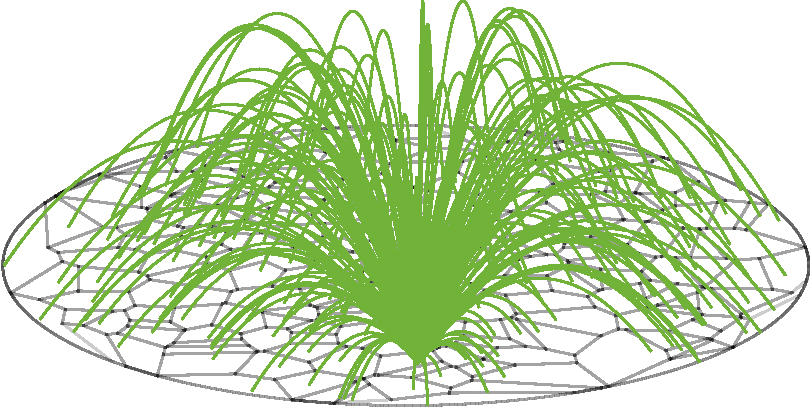
\includegraphics[width=0.4\textwidth]{gfx/chapter-monocentric/1.pdf}
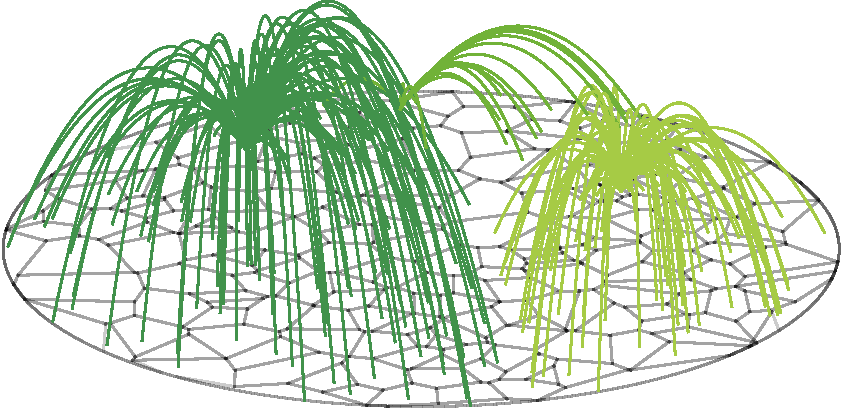
\includegraphics[width=0.4\textwidth]{gfx/chapter-monocentric/2.pdf}
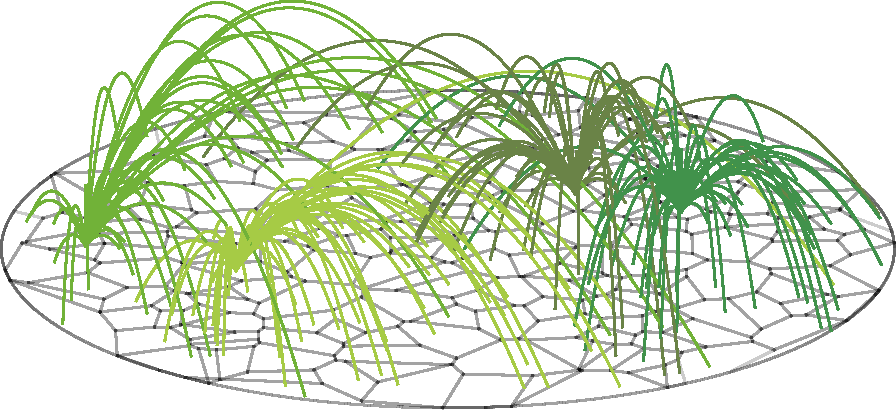
\includegraphics[width=0.4\textwidth]{gfx/chapter-monocentric/3.pdf}
\caption{The monocentric (top), distance-driven polycentric (middle)
  and attractivity-driven polycentric (bottom) regimes as produced by
  our model. Each link represents a commuting journey to an activity center. \label{fig:model_results}}
\end{figure}


From now on, we will assume that $\ell$ is large enough so that a
monocentric state exists for small values of the population. In this
regime, the value of $\eta$ prevails and the monocentric state evolves
to an attractivity-driven polycentric structure as the population
increases (if $\ell$ is too small, the monocentric regime does not
exist-see the Supplementary material~\cite{SM} for more details on
these points).  Starting from a small city with a monocentric
organisation, the traffic is negligible and $Z_{ij}\approx \eta_j$
which implies that all individual are going to choose the most
attractive center (with the largest value of $\eta_j$, say
$\eta_1$). When the number $P$ of households increases, the traffic
will also increase and some initially less attractive centers (with
smaller values of $\eta$) might become more attractive, leading to the
appearance of new subcenters characterized by a non-zero number of
commuters. More precisely, a new subcenter $j$ will appear when for an
individual $i$, we have $Z_{ij}>Z_{i1}$. The traffic so far is
$T(1)=P$ and $T(j)=0$ which leads to the equation
\begin{equation}
\eta_j-\frac{d_{ij}}{\ell}>\eta_1-\frac{d_{i1}}{\ell}\left[1+\left(\frac{P}{c}\right)^\mu\right]
\end{equation}
We assume that there are no spatial
correlations in the subcenter distribution, so that we can make the
approximation $d_{ij}\sim d_{i1}\sim L$. The new subcenter will thus
be such that $\eta_1-\eta_j$ is minimum implying that it will have the
second largest value denoted by $\eta_j=\eta_2$. For a uniform distribution
(details of the calculation can be found in the Supplementary
Material~\cite{SM}, section 2), on average
$\overline{\eta_1-\eta_2}\simeq 1/N_c$ leading to a critical value for
the population
%
\begin{equation}
P^*= c \left( \frac{\ell}{L N_c} \right)^{1/\mu}
\end{equation}
%
Whatever the system considered, there will therefore \emph{always} be
a critical value of the population above which the city becomes
polycentric (which can be smaller than one, in which case there is no
monocentric regime at all, see the Supplementary Material~\cite{SM}). The monocentric regime is therefore fundamentally
unstable with regards to population increase, which is in agreement with the fact that no major city in
the world exhibits a monocentric structure. We note that the smaller
the value of $\mu$ (or larger the value of the capacity $c$), the
larger the critical population value $P^*$ which means that cities
with a good road system capable of absorbing large traffic display a
monocentric structure for a longer period of time.


Having established that cities will eventually adopt a polycentric
structure, we can wonder how the number of subcenters varies with the
population. We compute the value of the population at which 
the $k^{th}$ center appears. We still assume that we are in the attractivity-driven regime and that, so far, $k-1$
centers have emerged with $\eta_{1} \geq \eta_{2} \geq ... \geq
\eta_{k-1}$~\cite{SM}, with a number of commuters $T(1), T(2), ...,
T(k-1)$, respectively. The next worker $i$ will choose the center $k$ if
\begin{equation}
Z_{ik} > \max_{j \in \left[1,k-1\right]} Z_{ij}
\end{equation}
which reads
\begin{equation}
\eta_k - \frac{d_{ik}}{\ell} > \max_{j \in \left[1,k-1\right]} \left\{
\eta_j - \frac{d_{ij}}{\ell} \left[ 1 + \left(
  \frac{T(j)}{c}\right)^\mu\right] \right\}
\end{equation}
The distribution of traffic $T(j)$ is narrow~\cite{SM}, which means that all the centers have roughly the same number of
commuters $T(j) \sim P/(k-1)$. As above we also assume that the
distance between the workers' households and the activity centers is
typically $d_{ij} \sim d_{ik} \sim L$. The previous expression now
reads
\begin{equation}
\frac{L}{\ell} \left( \frac{P}{(k-1)\,c} \right)^{\mu} > \max_{j \in
  \left[1,k-1\right]} \left( \eta_j \right) - \eta_k
\end{equation}
Following our definitions, $\max_{j \in \left[1,k-1\right]} \left(
\eta_j \right) = \eta_1$. According to order statistics, if the
$\eta_j$ are uniformly distributed, we have on average
$\overline{\eta_1 - \eta_k} = (k-1)/(N_c+1)$. It follows from these
assumptions that (1) the $k^{th}$ center to appear is the $k^{th}$ most attractive one (2) the average value of the population $\overline{P}_k$ at
which the $k^{th}$ center appears is given by:
%
\begin{equation}
\overline{P}_k = P^* \left( k-1 \right)^{\frac{\mu+1}{\mu}}
\label{eq:prediction}
\end{equation}
%
Conversely, the number $k$ of subcenters scales sublinearly with population as
\begin{equation}
k \sim \left( \frac{\overline{P}}{P^*} \right)^{\frac{\mu}{\mu + 1}}
\end{equation}
It is interesting to note that this result is robust: the dependence
is sublinear, \emph{whatever the distribution} of the random variable
$\eta$ (see the Supplementary Material~\cite{SM} for a discussion on this
point). We can therefore conclude that, probably very generally and
under mild assumptions, the number of activity subcenters in urban
areas scales sublinearly with their population where the prefactor and
the exponent depend on the properties of the transportation network of
the city under consideration. 

A previous study~\cite{Samaniego:2008} showed that the daily total
miles driven daily in a city --- the `total commuting
distance'---scales with the population as $L_{tot} \sim P^\gamma$
where $\gamma \in \left] 0.5, 1\right[$, which the authors interpreted
as cities having neither a neither totally centralized nor totally
decentralized structure. We can discuss this result within the
framework of our model in the following way. If the system was in the
pure attractivity-driven regime, we would have $L_{tot} \sim P$. But, if we
assume that we are in an intermediate regime where
Eq.~\ref{eq:prediction} holds, and where the system exhibits spatial
coherence~\cite{SM}, we can write the total length of commuting
journeys as
%
\begin{equation}
L_{tot} \sim P \frac{L}{\sqrt{k}}
\end{equation} 
%
Inverting the result from Eq.~\ref{eq:prediction} we therefore get
%
\begin{equation}
L_{tot} \sim P^{1-\frac{\beta}{2}}
\label{eq:beta}
\end{equation}
%
where $\beta = \frac{\mu}{\mu+1} \in \left[0 , 1\right]$. Our model is
thus consistent with the fact that the total traveled miles scales with
population with a non-trivial exponent comprised in $[0.5,1]$.\\


\begin{figure*}
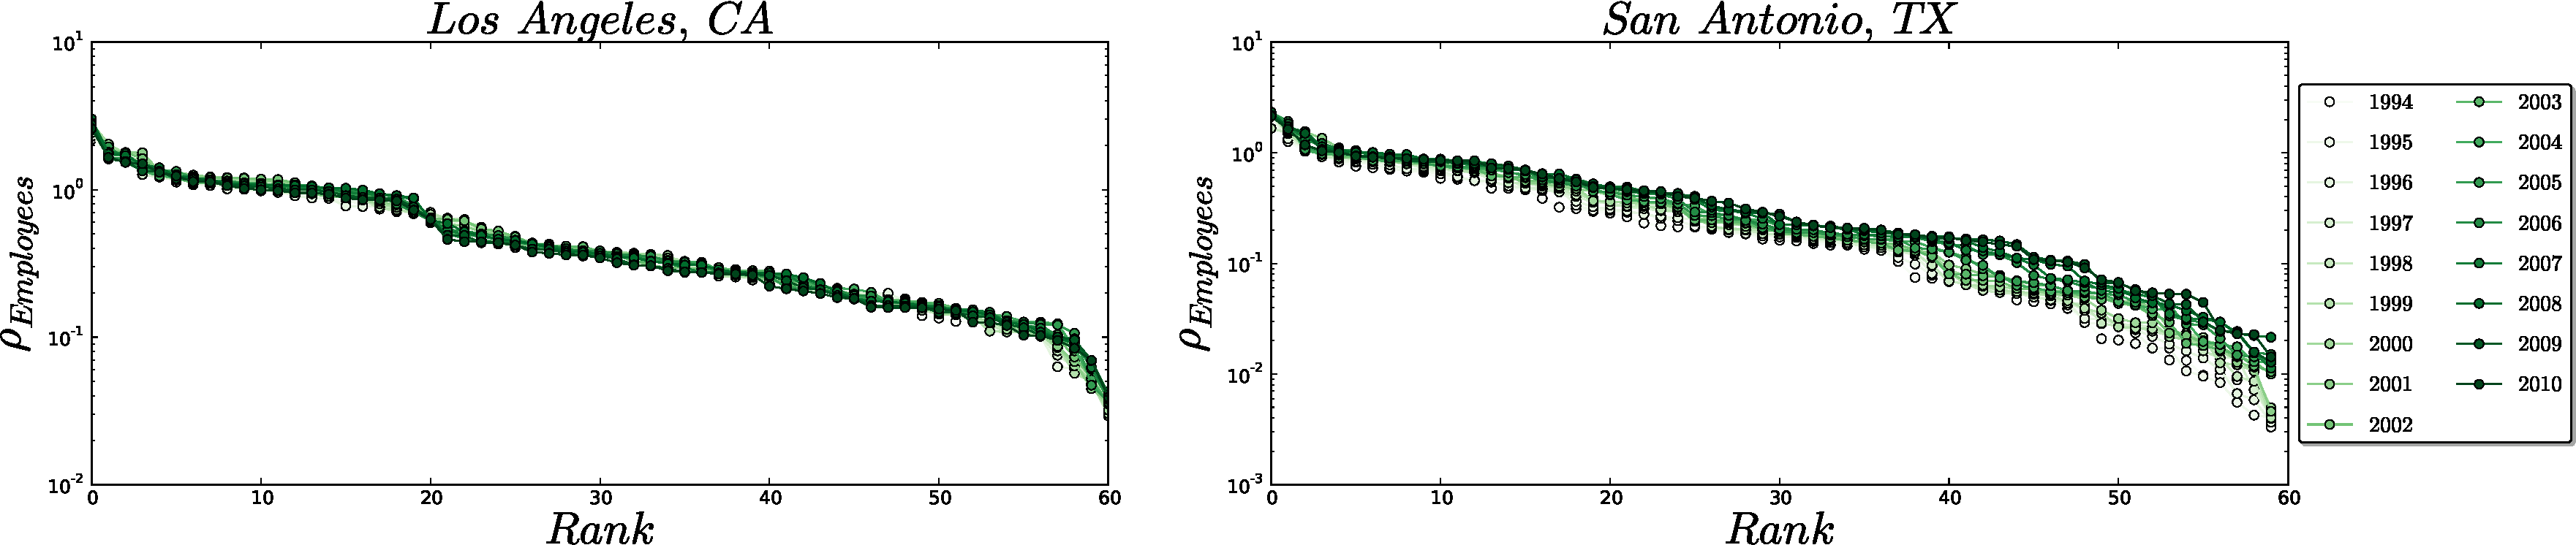
\includegraphics[width=\textwidth]{gfx/chapter-monocentric/4.pdf}
\caption{Rank-plot for the employment density (in employees per
  $km^2$) in Los Angeles, CA (left) and San Antonio, TX (right)
  between 1994 and 2010. See the Supplementary Material~\cite{SM} for more details. \label{fig:rank_plots}}
\end{figure*}

    \subsection{Empirical verification}
    \label{sub:empirical_verification}
    
People from the Census Bureau use the 2000 Census tract-to-tract commuting data
in order to get the employment density~\cite{Marlay:2010}. Use these data in
order to assess the employment density in 2000 MSAs. Use population data at the
same level in order to assess population density in 2000 MSAs.
Plot at several levels of the threshold and show the many different centers.
Propose a method to compute the number of centers (exponential, Loubar...).\\
        \subsubsection{Counting the number of centers}
        \label{ssub:counting_the_number_of_centers}
        
        
We now test the prediction given by Eq. (\ref{eq:prediction}). For
that purpose, we collected data for the number of employees per Zip
Codes in the United States for 16 years, between 1994 and
2010~\cite{ZBPdata}, as well as the population of all cities in the US
between 1994 and 2010~\cite{CensusData}. We estimate the number of
subcenters by constructing the rank-plot of the employment density
$\rho$ (number of employees per $km^2$) for each Zip Code of a given
urban area~\cite{Griffith:1981,Dokmeci:1994}. These plots display a decay as fast as an exponential
(Fig.~\ref{fig:rank_plots}) which implies that there exists a natural
scale for the rank, that we interpret here as the typical number of
activity centers. It also implies that any reasonable method should
give an estimate of the number of subcenters of the same order of
magnitude (which would not be the case for slowly decaying function
such as power laws for example). We first note that for some cities
--typically large ones with stable populations
(Fig.~\ref{fig:rank_plots}, left)-- the employment spatial statistics
remained stable over the period of study. For other cities, we observe
large variation of the number of subcenters
(Fig.~\ref{fig:rank_plots}, right). We then plot (Fig.~\ref{fig:data})
the population $P$ of cities (with population $P>100$) versus the
estimated number of subcenters $k$ (the dispersion in the scatterplot
probably results from the fact that different cities have different
resilience levels to congestion). On average, we observe a power law
dependance with exponent $\delta=1.56 \pm 0.15$ (the result is robust
with regards to the estimate of $k$, see the Supplementary
Material~\cite{SM} for more details). Inverting this relation gives us
the number of subcenters as a function of the population
%
\begin{equation}
k \sim P^{\beta}
\end{equation}
%
with $\beta \sim 0.64$. This result is strikingly in agreement with
the prediction given by our model: the number of subcenters in a city
scales sublinearly with its population.\\

\begin{figure}
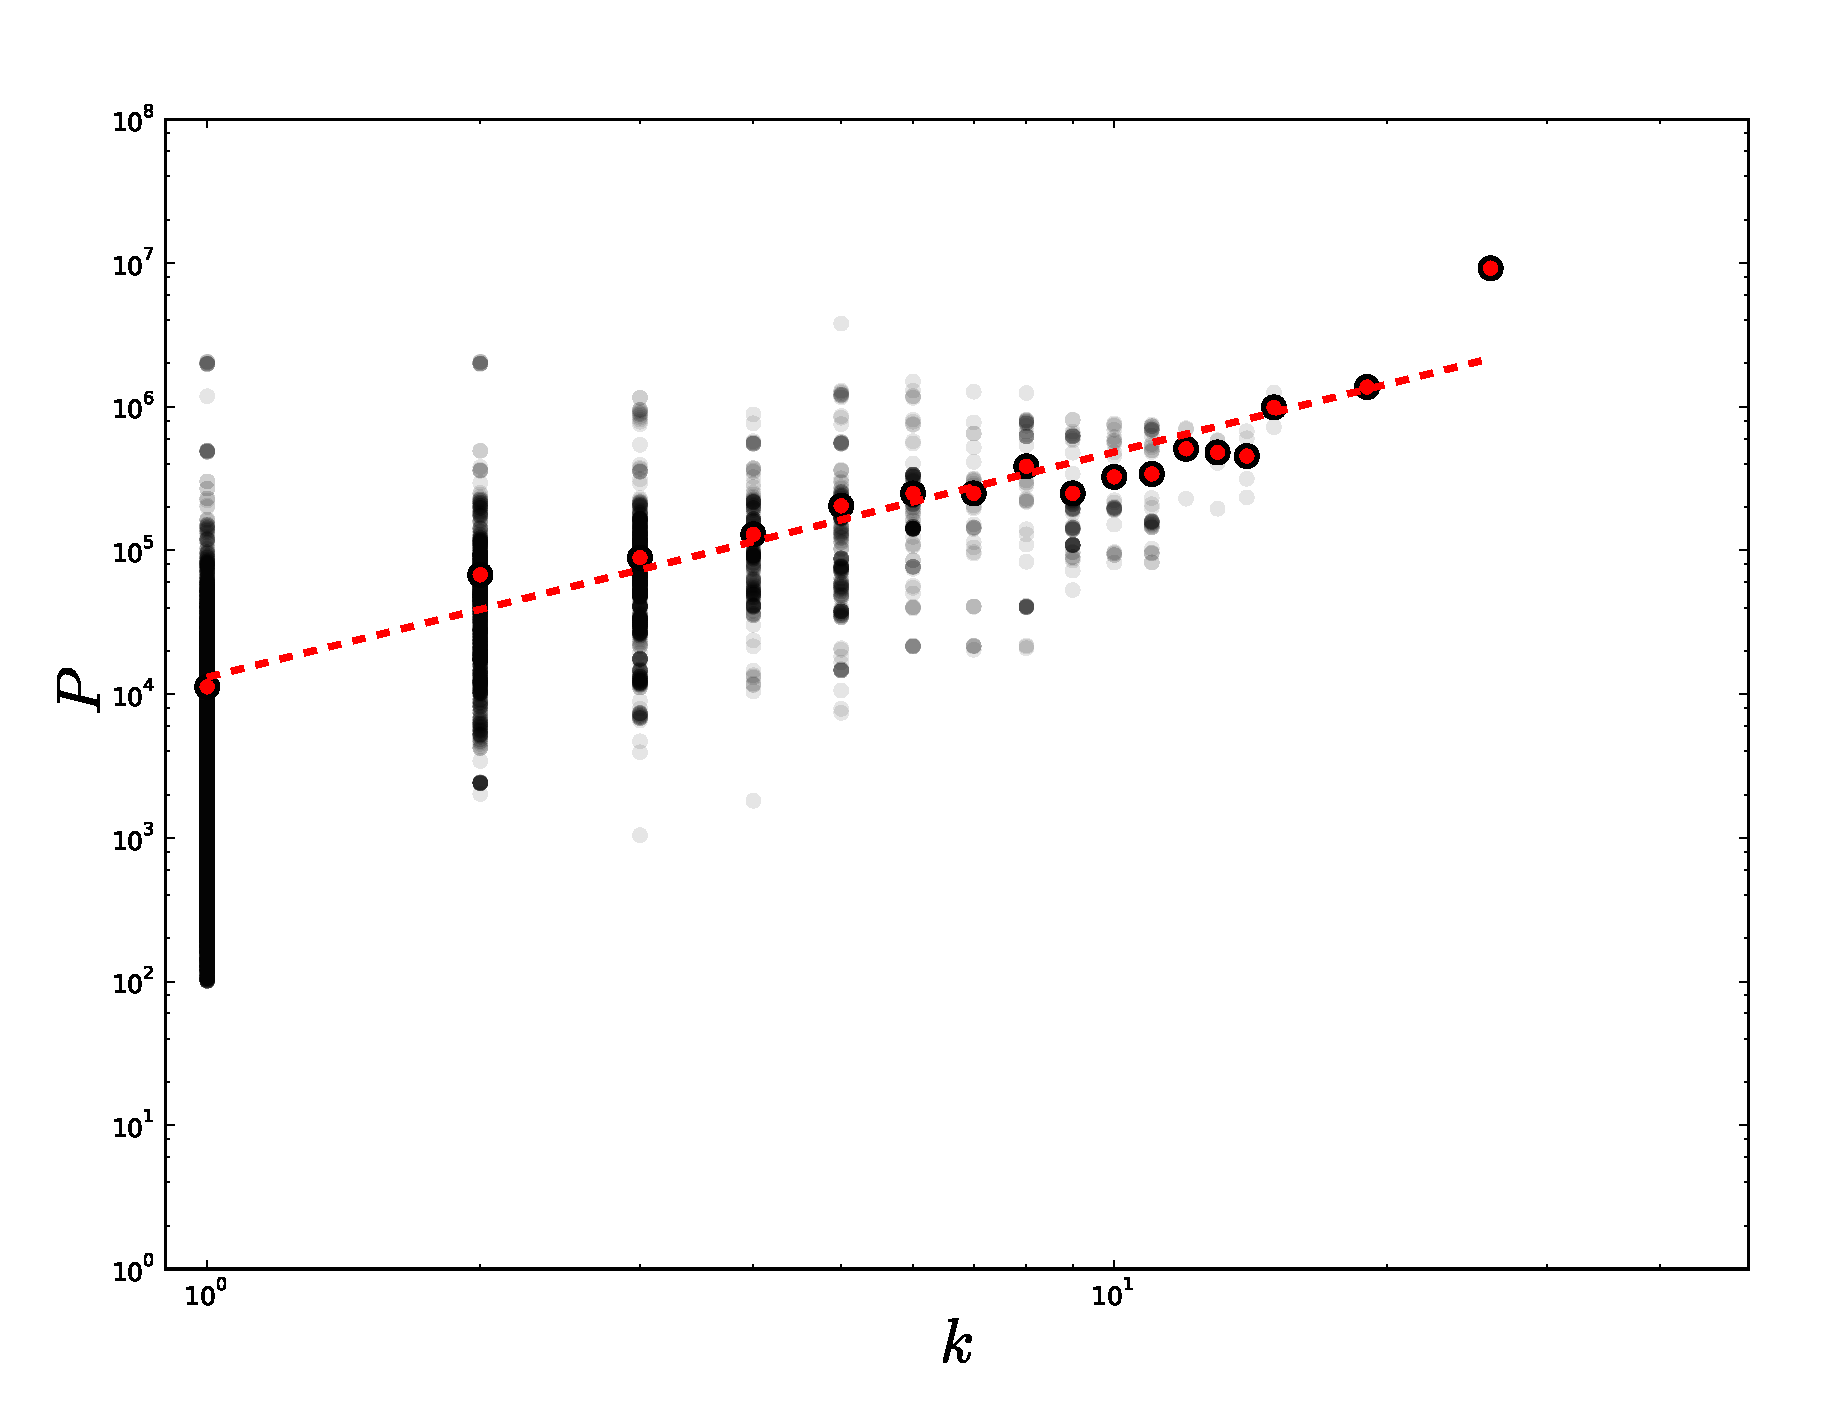
\includegraphics[width=0.5\textwidth]{gfx/chapter-monocentric/5.pdf}
\caption{Scatter plot of the estimated number of subcenters versus the
  population for about 9000 cities with population over 100 people in
  the US. The red dots represent the average population for a given
  number of subcenters. We fit this average with a power-law
  dependence (represented by a red dashed line) giving an exponent
  $\delta=1.56\pm 0.15$ ($r^2=0.87$). See the Supplementary Material~\cite{SM} for more details on the computation of $k$ and the robustness of the results. \label{fig:data}}
\end{figure}

Using the measured value of $\beta$ and Eq. (\ref{eq:beta}) we can estimate the exponent of
the scaling of $L_{tot}$ with the population and find $L_{tot} \sim
P^{\,0.68}$ which agrees very well with the value $0.66$ measured
in~\cite{Samaniego:2008} directly on the data of the daily total miles
driven in more than $400$ cities in the US.\\

While agglomeration economies seem to be the basic process explaining
the existence of cities and their spectacular resilience, this study
brings evidence that congestion is the driving force that tears them
apart. The non trivial spatial patterns observed in large cities can
thus be understood as a result of the interplay between these
competing processes. We believe that the present model represents an
important step towards a quantitative, predictive science of
cities. More generally, this microscopic approach is an interesting
example of an out-of-equilibrium model: it is governed by local
optimization with saturation effects, leads to different regimes, and
is characterized by non-trivial dynamical exponents. In this respect,
we believe that this discrete approach might be of use in the study of
pattern formation in biology --which have been so far explored from a
global optimisation perspective~\cite{Ashton:2005} or using
coarse-grained reaction-diffusion approaches with density dependent
diffusion coefficients~\cite{Cates:2012}-- to compute quantities that
are out of reach within the current methods.
\section{Proviso}
\label{sec:proviso}


 % Chapter 2

%------------------------------------------------

\ctparttext{Scaling of indicators with the population size of the city has been
recently re-discovered and explored by the different communities. In this part,
the contribution are threefold. First, a review of the exisiting literature,
pre- and post-2007 on scalings and their interpretation. Then, a model to
explain the scaling of several indicators related to mobility in cities. We then
discuss some results, Zahavi's constant and Newman and Kenworthy's famous curve.
Finally, we show that scalings pose the question of how we should define cities
as systems.} % Text on the Part 2 page describing the content in Part 2

\part{Scaling in cities} % Second part of the thesis

% !TEX root = ../thesis-example.tex
%
\chapter{Scaling in cities}
\label{sec:scaling_in_cities}

\begin{flushright}{\slshape    
The allometric law promises to become\\
an integral part of geography theory.} \\ \medskip
--- David Harvey (1969)~\cite{Harvey:1969} 
\end{flushright}

\cite{Pumain:2004} Paper while Pumain was at the Santa Fe institute.

\section{Introduction}
\label{sec:introduction}

    \subsubsection{Measures}
    \label{ssub:measures}

\paragraph{Area versus population} \cite{Stewart:1947} is the first occurence of
the scaling area versus population, specified in the \cite{Stewart:1958}. \cite{Boyce:1963} also does that with census
data. \cite{Nordbeck:1965} is the first occurence
of allometric scaling called that way, with explicit reference to biology (not
read, have to trust Tobler on that one).
\cite{Tobler:1969} first confirmation using satellites. \cite{Nordbeck:1971} for
an obtainable article. More recently appears in ~\cite{Guerois:2003}.
\cite{Batty:2011} reviews the measures done in the past.

\paragraph{Economic diversity} \cite{Zipf:1949} Zipf has it (check). \cite{Berry:1967} Berry has the scaling I
believe, on the number of functions fulfilled by a city. \cite{Pumain:2006} it
is the basis of her theory. \cite{Bettencourt:2014}

\paragraph{Wealth} \cite{Bettencourt:2007} in form of the GDP.
\cite{Bettencourt:2014} employment proportional to population.

\paragraph{Human interactions} \cite{Schlapfer:2014}

\paragraph{Mobility} \cite{Samaniego:2008} total number of miles driven vs
population (cities neither centralized not decentralized).
\cite{Bettencourt:2007} gasoline sales. $CO_2$ in \cite{Fragkias:2013,
Oliveira:2014, Rybksi:2013}.

\paragraph{Infrastructure} \cite{Veregin:1997} number of edges versus population.
\cite{Samaniego:2008} Lane miles versus population. \cite{Bettencourt:2007}
cable length.

\paragraph{Living Stuff} \cite{Bettencourt:2007} water consumption, electrical
consumption, total housing.

    \subsubsection{Theory}
    \label{ssub:theory}
    
\cite{Pumain:2006} for an interpretation of scaling laws in terms of
innovation waves etc.

\cite{Bettencourt:2013} for the latest model to date.


\subsection{What can scalings tell us about cities and systems of
cities?}
\label{sub:what_can_scalings_tell_us_about_cities_and_systems_of_cities_}

\paragraph{On cities} Scalings are, by essence, cross-sectionnal studies of cities. Scaling studies
and their conclusions are usually structured around several assuptions. The
first assumption, implied by the use of city population as the dependent
variable, is that the population count of a city (and not its surface area, or the
number of buildings, the length of its streets, etc.) is the appropriate variable to
account for its size. The second assumption, never really stated, is that the
processes responsible for the city-wide value of the quantity being studied
occur over time-scales that are at most of the same order of the time-scales
over which population changes. A very fast increase in population size, for
instance, is not likely to be immediately reflected in terms of the length of
streets, for instance. Of all the deviations measured by Bettencourt et al, it
is difficult to say whether these deviations account for a real over or
under-performance of the city compared to the other cities in the system, or
just for the time-delay in the studied quantity to react to population
changes. In fact, these questions cannot be answered until we understand the
evolution of these quantities in time.

\paragraph{On systems of cities} The fact that we observe scalings when taking a
single country into account, and a cloud of points when mixing two different
countries, is a signature of the integration of cities into systems of
cities. Although it is not clear at the moment what are the mechanisms
reponsible for the 'equilibration' of the scaling there clearly is an
adjustement that is being made, because the economy, the population, etc. are
tightly connected through the flow of commodities, populations, information and
funds.

\paragraph{And the ergodic counter-argument?} Pumain in... argues that
transversal averages are usable to describe the time-evolution of individual
cities if and only if the trajectories of cities are egodic (which they clearly
aren't). This argument is misguided, and based on several misunderstandings of
what scalings represent, and the role of ergodicity in physical theories.
Although prompt to deplore the lack of knowledge of the existing geography
literature physicists have, we have to deplore on our side the improper use of
several concepts borrowed from physics, and the sometimes improper use of
mathematics and the latest developpements in some branches of physics (network
theory for instance). This is not an attack, this is just to point out that no
side is free form reproaches, and time wasted on criticising one another for
improper use of the literature would be put to better use if spent on teaching
these things to one another.

\section{From mobility patterns to scaling}
\label{sec:from_mobility_patterns_to_scaling}


The recent availability of data for cities has allowed scientists to exhibit scalings which present themselves in the form of a power-law dependence on population of various socio-economical and structural indicators. We propose here a stochastic theory of urban growth which accounts for some of the observed scalings and we confirm these predictions on US and OECD empirical data. In particular, we show that the dependence on population size of the total number of miles driven daily, the total length of the road network, the total traffic delay, the total consumption of gasoline, the quantity of $CO_2$ emitted and the relation between area and population of cities, are all governed by a single parameter which characterizes the sensitivity to congestion. Our results suggest that diseconomies associated with congestion scale superlinearly with population size, implying that --despite polycentrism-- cities whose transportation infrastructure rely heavily on traffic sensitive modes are unsustainable.



The recent availability of an unprecedented amount of data has made possible quantitative studies of cities~\cite{Fujita:1999,Batty:2007,Marshall:2004}, opening the way to a Science of Cities. In particular, the discovery of allometric scaling relationships in cities has driven the quantitative research on urban systems in the past years. Indeed, there is a great amount of evidence to show that different socio-economic indicators in cities, such as the GDP, the crime rate, the number of patents as well as different structural indicators such as the total length of the road network, the urbanized land area, etc., exhibit robust scaling relationships with respect to population~\cite{Newman:1989,Makse:1995,Pumain:2006,Bettencourt:2007,Samaniego:2008,Rozenfeld:2008,Pan:2013}. The existence of these simple scaling relationship hints at the existence of universal processes shared by urban systems, and thus at the possibility of modeling cities.\\

A common trait shared by all complex systems --including cities-- is the existence of a large variety of processes occuring over a wide range of time and spatial scales. The main obstacle to the understanding of these systems therefore resides in uncovering the hierarchy of processes and in singling out the few ones which govern their dynamics. Albeit difficult, the hierarchisation of processes is of prime importance. A failure to do so leads to models which are  either too complex to give any real insight into the phenomenon, or too simple and abstract to have any resemblance with reality. As a matter of fact, despite numerous attempts~\cite{Fujita:1982,Makse:1995,Batty:2008,Frasco:2013,Bettencourt:2010,Bettencourt:2013}, a theoretical understanding of many observed empirical regularities in cities is still missing.\\

In the present study, we show that the spatial structure of the mobility pattern controls the behaviour of many quantities in urban systems. Indeed, cities are not only defined by the spatial organisation of places fulfilling different functions --shops, places of residence, workplaces, etc.-- but also by the way indivduals move among them. Understanding where people live, where and how they travel within the city thus appears as a necessary step towards a scientific theory of cities.\\ 

Although an increasing amount of data about mobility is now available~\cite{Gonzalez:2008}, we still lack a simple model explaining the dominant mechanisms governing the formation and evolution of mobility patterns. Many factors such as geographical constraints, facilities location and available transportation --to name a few-- can impact the mobility and it thus appears as an intricate issue. Here, we tackle the problem of mobility by making simplifying --yet not simple-- assumptions, trying to grasp the most important parameters which define the problem. We thus build upon a simple out-of-equilibrium model previously developed~\cite{Louf:2013}. This model, among other things, accounts for the polycentric transition of cities and gives a prediction for the number of centers as a function of population. We show that this framework allows us to predict the behaviour of many quantities related to mobility and the structure of cities: the scaling with population of the total time wasted in congestion, transport related $CO_2$ emissions, total travelled distance, total lane miles and surface area.

Our results allow us give a quantitative insight into two important debates around urban systems. First, we are able to discuss the benefits of polycentricity and quantify some of its aspects. Then, maybe more importantly, we are able to put into perspective the sustainability of urban systems.


\subsection{Naive scalings}

We start by presenting some naive arguments to estimate the scaling exponents for the area $A$, the total daily distance driven $L_{tot}$ and the total lane miles $L_N$. Although these predictions turn out to be wrong, naive scalings are useful as a first approach to the problem as they allow us understand how the different quantities relate to one another.


\subsubsection{Surface area} 

First, we would like to estimate the dependence of the area $A$ of a city on its population $P$ --a long standing problem in the field~\cite{Makse:1995}. A first crude approach would be to assume that cities evolve in such a way that their population density $\rho = P/A$ remains constant. This assumption straighforwardly implies that the area should scale linearly with population
%
\begin{equation}
A \sim \lambda^2\, P
\label{eq:area_naive}
\end{equation}

where $\lambda^2$ is the average surface occupied by each individual (the assumption of a constant density is then equivalent to the one of a constant average surface per capita).

\subsubsection{Total length of roads} 

We would now like to estimate the total length $L_N$ of all the roads within a city. If we consider that the network formed by streets is such that all the nodes (intersections) are connected to their closest neighbour, the typical length of a road segment is given by

\begin{equation}
\ell_R \sim \sqrt{\frac{A}{N}}
\end{equation}

where $N$ is the number of intersections. Previous studies of road networks in different regions, and over extended time periods~\cite{Strano:2012,Barthelemy:2013}, have shown that the number of intersections is proportional to the population size. Therefore, the typical length of a road segment (between two intersections) varies with the population size $P$ as
%
\begin{equation}
\ell_R \sim \sqrt{\frac{A}{P}}
\end{equation}
%
and the total length of the network $L_N \sim P\ell_R$ should then scale as
%
\begin{equation}
\frac{L_N}{\sqrt{A}}\sim\sqrt{P}
\end{equation}
%
Using the naive scaling for the dependence of $A$ on population size given previously in Eq.~\ref{eq:area_naive} we finally get
\begin{equation}
L_N \sim P
\end{equation}


\subsubsection{Total daily commuting distance} 

\paragraph{Individual constraint} We would also like to estimate the total commuting distance $L_{tot}$. The first constraint on this distance comes from individuals's limitations and behaviour. We make here the simple assumption that individuals choose their residence and work place such that their total commuting distance is fixed (or at least smaller than a certain value) and equal on average to $\ell_C$. In that case, we would simply have
%
\begin{equation}
  \frac{L_{tot}}{P} \sim \text{const.} = \ell_c
\label{eq:assum}
\end{equation}
(by constant, we mean independent from the population size of the city).

\paragraph{The city structure constraint} An additional contraint on $L_{tot}$ is given by the structure of the city~\cite{Samaniego:2008}. Indeed, the individual commuting distance is also related to the total suface area of the city and the location of activity centers.

If we first assume that the city is monocentric, individuals are all commuting to the same center and the typical commuting distance $\ell^m_c$ is controlled by the typical size of the city of order $\sqrt{A}$ 
%
\begin{equation}
\frac{L_{tot}^{m}}{\sqrt{A}} \sim P
\end{equation}

On the other hand, if we assume that the city is completely decentralized, the typical commuting distance is of order the nearest neighbour distance $\sqrt{A}/\sqrt{P}$, and we obtain
%
\begin{equation}
\frac{L_{tot}^{d}}{\sqrt{A}} \sim \sqrt{P}
\end{equation}


\subsection{Comparison of naive scalings with empirical results}

The comparison of the naive exponents with the exponents measured on US data is shown in Table 1 (see the Methods section for details about the data). There are important discrepancies, which we discuss in the following.

First, we note that the naive scaling for the surface area $A$ predicts a value of the exponent that is quantitatively --and worse, qualitatively-- different from that observed. Indeed, we find that for real cities
%
\begin{equation}
A \sim P^{\,a}
\end{equation}
%
with $a=0.85$. While the naive argument implies a linear dependence of the surface area $A$ with population, we find a sublinear scaling in the data, which is a qualitatively different behavior (Table~\ref{table:naive}). This disagreement on this basic quantity will naturally impact the scaling of the other quantities.

%On the other hand, the prediction for $L_N / \sqrt{A}$ seems better, with an exposant close to the one observed. This %implies that the link between the network structure and the population is well captured by the naive argument. However, %the naive prediction for $L_N$ is incorrect: it predicts a linear dependence on population while data indicate a sublinear %behaviour. This confirms the problem with the naive prediction for the behaviour of $A$ that we discussed above.

The data also show that $L_{tot}/P$ can be considered reasonably independent from $P$ (with a value of approximately $23$ miles for the US, see Fig.~\ref{fig:LtotoverP}), in agreement with the individual constraint assumption (Eq. \ref{eq:assum}). This finding is also in agreement with the results drawn from census data in Germany by~\cite{Wilkerson:2013}. Although this assumption of a constant distance is simple and verified on the US data, we think that it deserves to be systematically tested on other datasets for other countries and cities. 
%
\begin{figure}
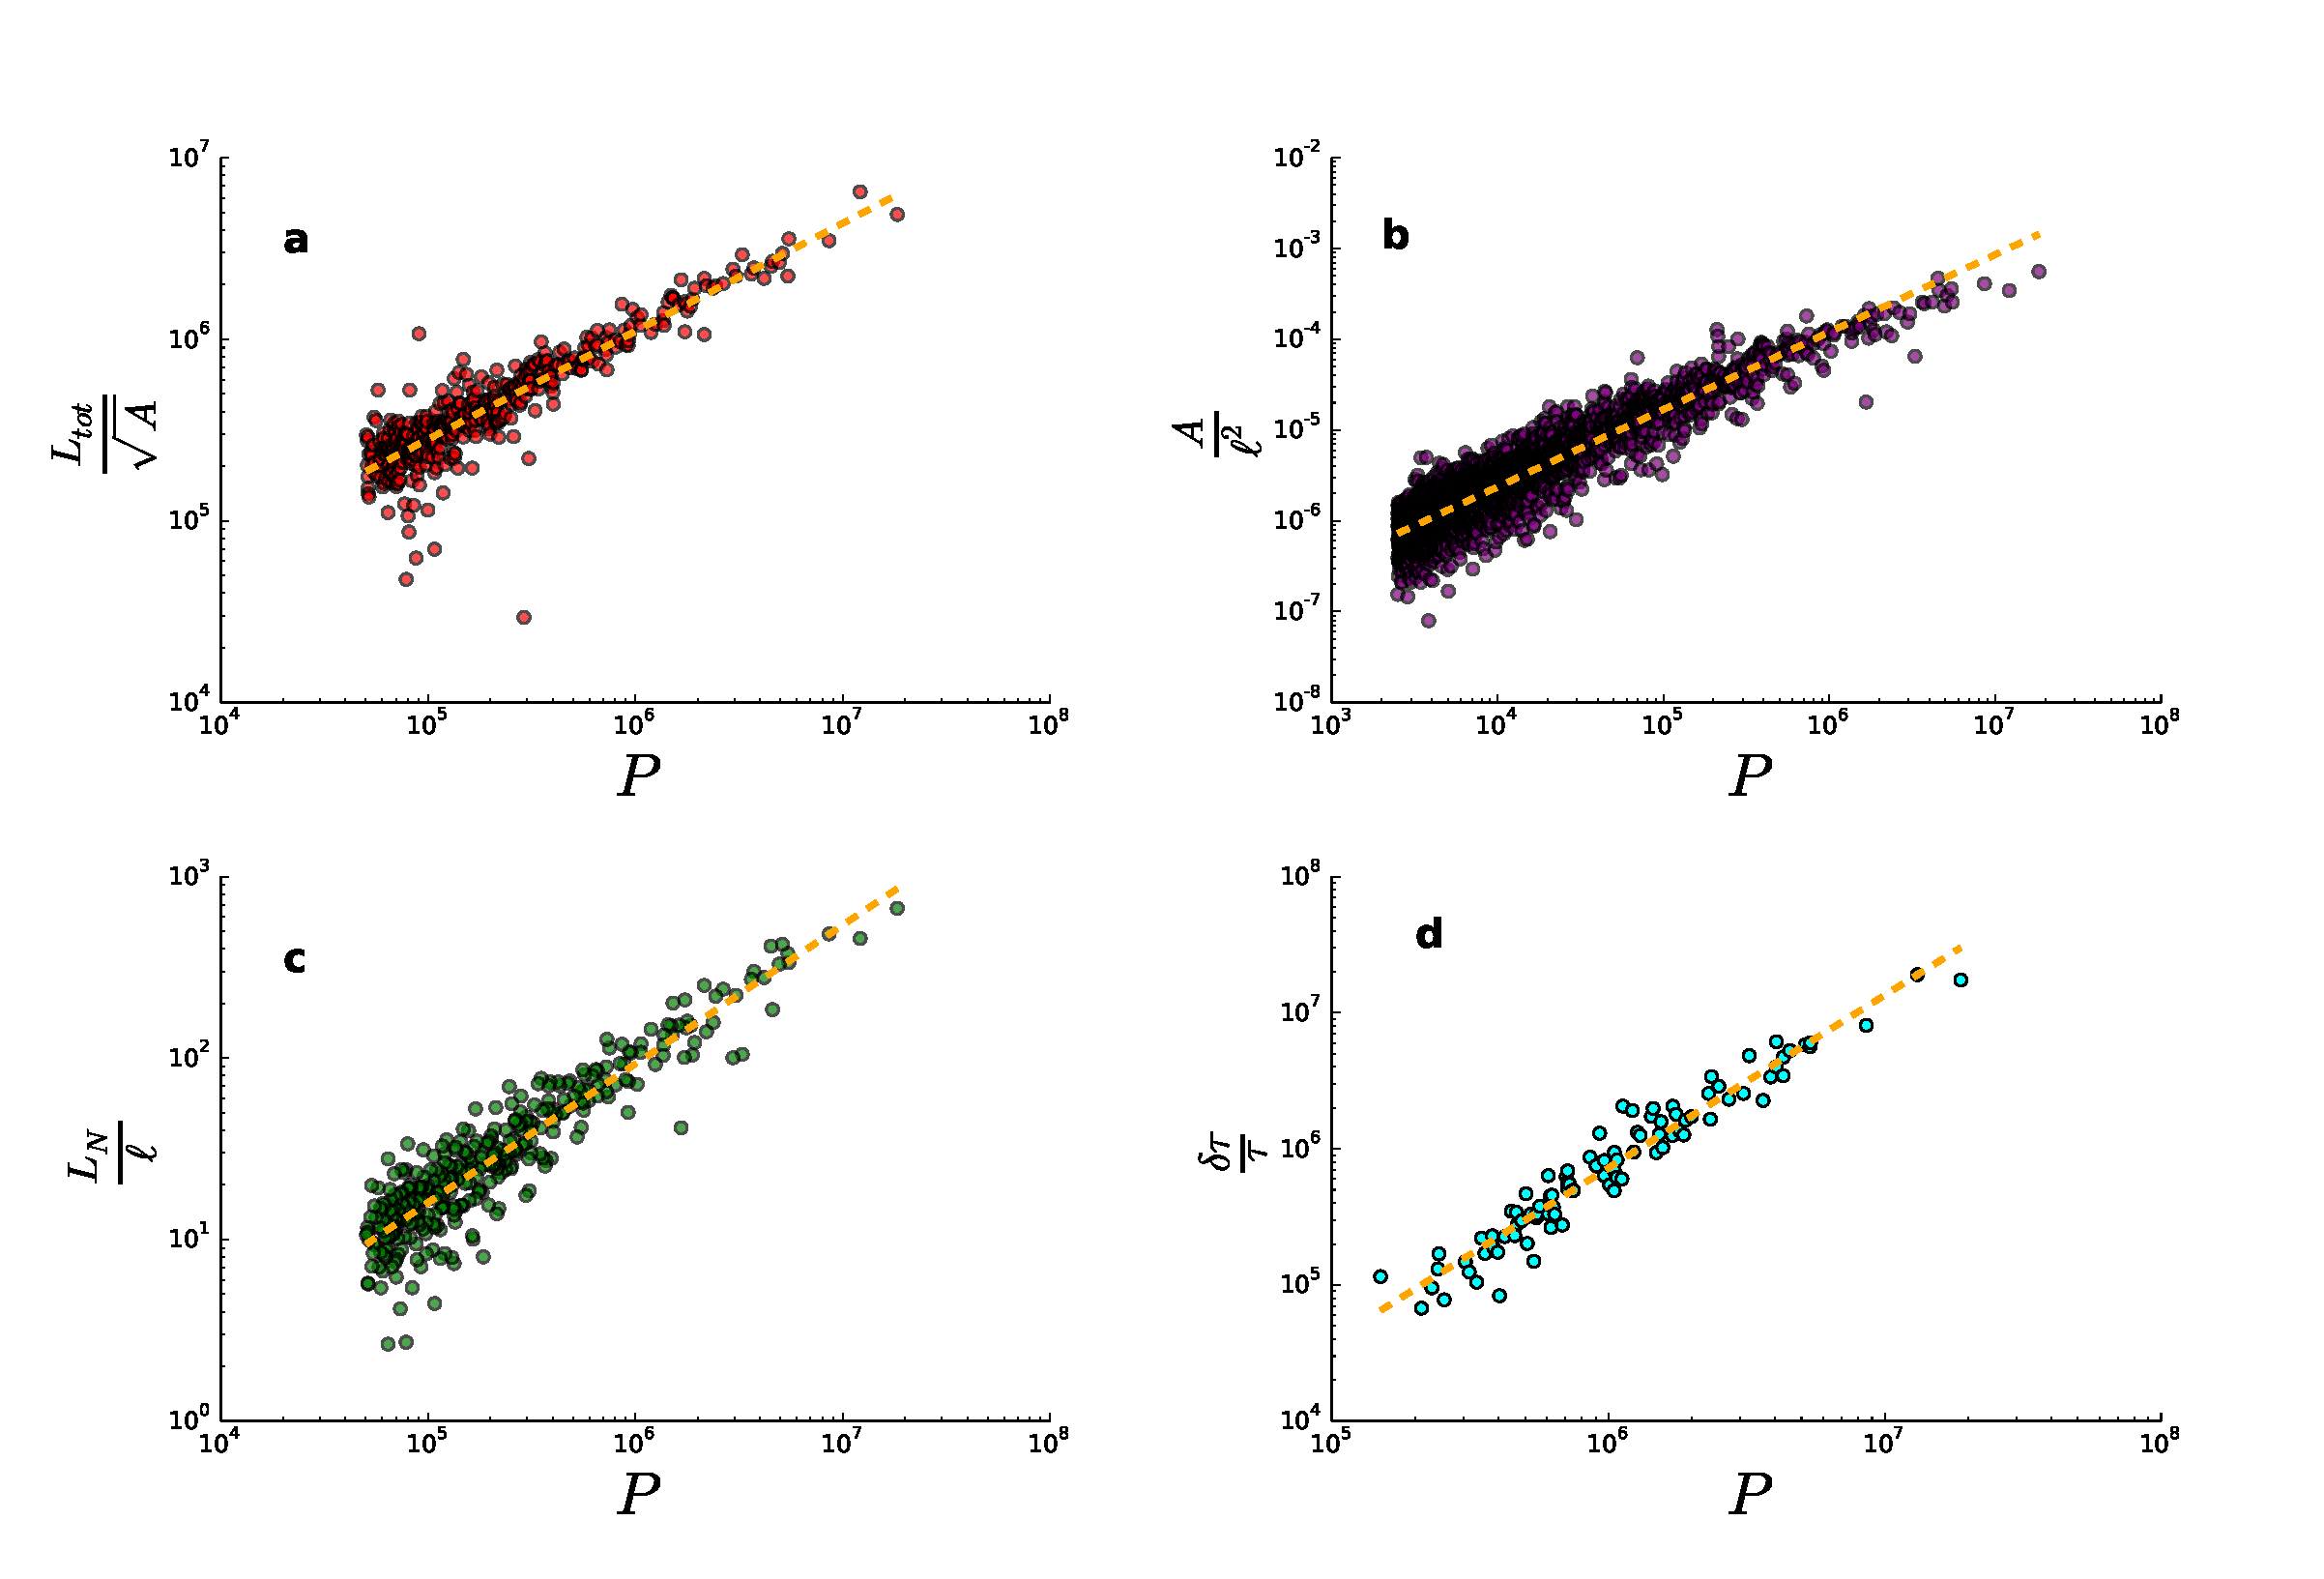
\includegraphics[width=1.0\textwidth]{gfx/chapter-scaling/figure_1.pdf}
\caption{Constant daily driven distance per capita. (a) daily total driven distance per capita as a function of population for 441 urbanised area in the US in 2010. The data shown in the plot are compatible with a population-independent behaviour. (b) Histogram of the daily total driven distance per capita for the same cities. The average daily driven distance for these cities is $23$ miles, and the standard deviation $7$ miles.}
\label{fig:LtotoverP}
\end{figure}


Finally, the scaling of $L_{tot}/\sqrt{A}$ given in the extreme cases of a monocentric city structure and a totally decentralized city structure disagree with the value measured on data (see Table~\ref{table:naive}). This suggests that most cities have a structure that is neither completely centralized, nor totally decentralized. In particular, this result cast some doubts about the study \cite{Bettencourt:2013} which assumes implicitely that cities are always monocentric.
Any situation between the two previous extreme cases would give a scaling of the form $L_{tot}/\sqrt{A}\sim P^{\,b}$ where $b \in [1/2,1]$. One can easily see that this expression is consistent with that of $A/\lambda^2$ and $L_{tot}/P$ if
%
\begin{equation}
b = 1-\frac{a}{2}
\label{eq:consis}
\end{equation}
%
which is indeed what we observe empirically (up to error bars). This preliminary analysis thus leads us to the conclusion that, in order to compute the various exponents, we need to better describe the structure of commuting patterns. In other words, we need to find a description of cities that goes beyond the naive monocentric or totally decentralized views, and which accounts for the observed sub-linear scaling of the surface area $A$.

% The choice of assumptions is crucial here and is essentially determined by the period considered, and the time scales associated with the evolution of the urban system. Mobility indeed depends on transportation means which evolved very rapidly during the last two centuries. Because the area of an urban system results from centuries of evolution, we do not a priori expect our model --where individual vehicles are assumed to be the only vector of mobility-- to give a prediction valid for all countries and all times. At the present stage, a full discussion about this problem and even the possibility of describing the time evolution of cities might seem within reach, but we leave it for further studies. 
\subsection{Beyond naive scaling: modeling mobility patterns}
%

We begin with the assumption that mobility patterns are mostly driven by the daily commuting and we would like to understand how an individual, given his household location,  will choose his job location. We assume that this choice will be determined by two dominant factors: the expected wage at a given job, and the commuting time to this job's location. Indeed, places with high average salaries are attractive, but having to spend a sensible amount of time commuting every day is less desirable. We assume there are $N_c$ potential activity centers in the city, each characterized by an average wage $w(j)$ at location $j$. This wage is endogenously determined and depends a priori on many factors such as agglomeration effects~\cite{Glaeser:2001}, the type of industry, etc. Although it is in principle possible to write down equations to determine the wage (as attempted in~\cite{Fujita:1982} for instance), not only is it impossible to solve them, but also not necessarily useful. A similar situation arises in physics when one studies the behaviour of atoms made of a large number of electrons. Physicists found out~\cite{Dyson:1962} that, in fact, a statistical description of these systems relying on random matrices could lead to predictions which agree with experimental results. We would like to import this idea of replacing a complex quantity such as wages --which depends on so many factors and interactions-- by a random one in spatial economics. So, we treat the wage \emph{as if} it was exogenous and random~\cite{Louf:2013}, that is we write $w(j)=s\,\eta_j$ where $s$ represents the typical income in this city and $\eta$ is a random number chosen uniformly in $[0,1]$. Furthermore, we assume that the commuting time does not only depend on the distance between the two places, but also on the traffic $T_{ij}$ between those two locations. An individual living at $i$ will thus commute to the center $j$ which corresponds to the best trade-off between income and commuting time, thus to the center $j$ such that the quantity
%
\begin{equation}
Z_{ij} = \eta_j - \frac{d_{ij}}{\ell} \left[ 1 + \left( \frac{T(j)}{c} \right)^\mu \right]
\end{equation}
%
is maximum~\cite{Louf:2013}. The quantity $d_{ij}$ is the euclidean distance between $i$ and $j$ (both supposed to be scattered randomly across the city), $T(j)$ the total incoming traffic at $j$, $c$ the capacity of the underlying transportation network, and $\mu$ is an exponent describing the sensitivity of the network to congestion. The quantity $\ell$ is the maximum distance that people can financially travel daily, defined as the ratio between the typical individual income and the transportation costs per unit of distance.\\

This simple model displays a surprisingly rich behaviour~\cite{Louf:2013}. In particular, it accounts for the monocentric to polycentric transition observed in most cities. It has been a well-known fact for quite some time that as cities grow, they evolve from a monocentric organisation where all the activities are concentrated in the same geographical area --usually the central business district-- to a more distributed, polycentric organisation~\cite{Fujita:1982,McMillen:2003}. Several theories in spatial economics exist~\cite{Fujita:1999}, but are not satisfactory for many reasons. Among other things, they do not take congestion into account and have no predictive, testable content~\cite{Bouchaud:2008}. Within this framework, congestion is actually responsible for the transition, and the number of activity centers in a city of population size $P$ is on average given by
%
\begin{equation}
k = \left( \frac{P}{P^*} \right)^{\frac{\mu}{\mu+1}}
\label{eq:num_centers}
\end{equation}  
with 
\begin{equation}
P^* = c \left( \frac{\ell}{\sqrt{A} N_c} \right)^{1/\mu}
\end{equation}

% Forgetting all the other variables but $A$ and $P$ we get

% \begin{equation}
% k \sim \left( P\,A^{1/2\mu}\right)^{\frac{\mu}{\mu+1}}
% \label{eq:num_centers}
% \end{equation}  

Using data of employment per Zip Code Area in the US~\cite{Louf:2013}, we showed that

\begin{equation}
k \sim P^{\,\alpha}
\end{equation}

where we measure $\alpha = 0.64 \pm 0.12$ ($95\%$ confidence interval (CI)). In other words, the number of centers scales sublinearly with population size. 


% We now show how the polycentric structure that emerges from the existence of congestion controls the dependence of the surface area on population. 
%
\begin{figure*}
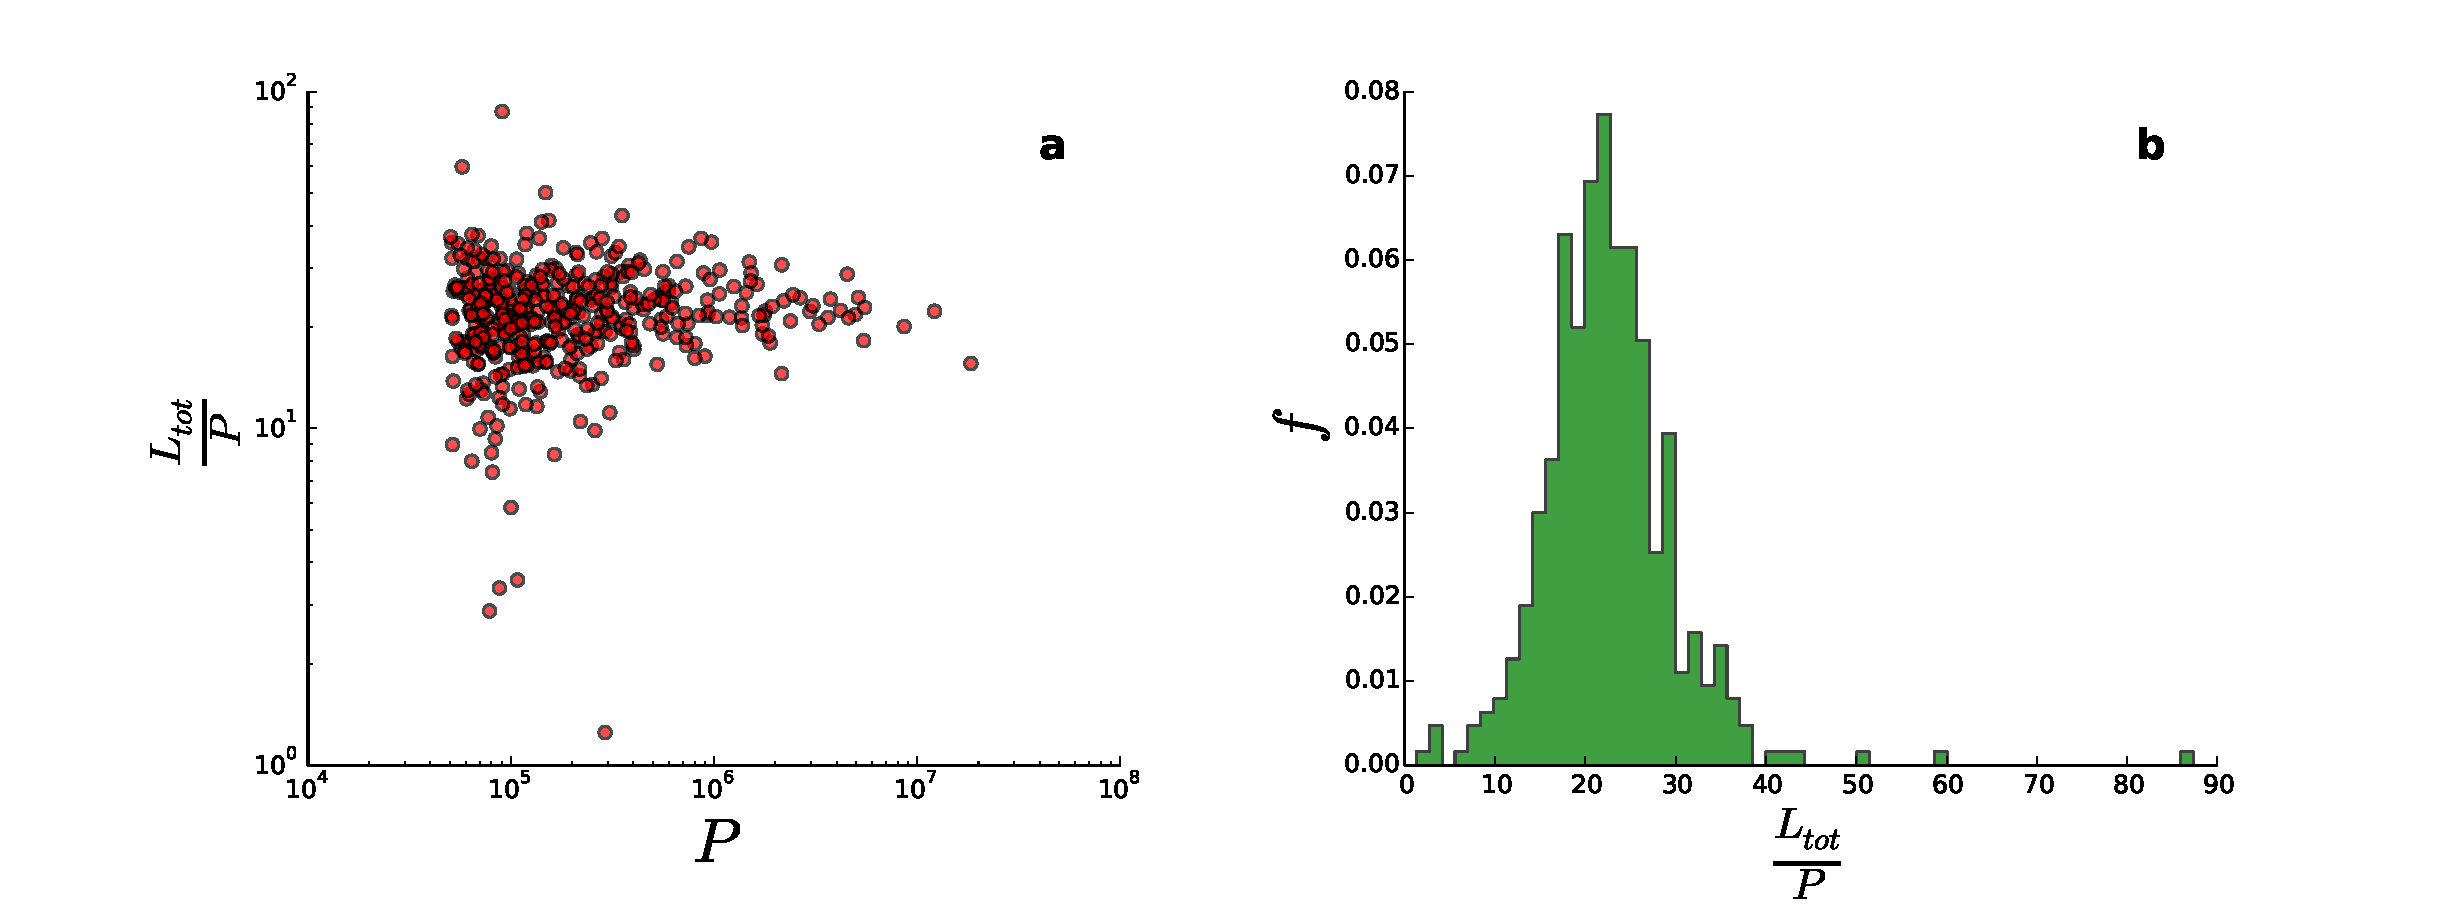
\includegraphics[width=1.0\textwidth]{gfx/chapter-scaling/figure_2.pdf}
\caption{Mobility and city structure and their impact on agglomeration economies and diseconomies. (a) Variation of the daily total driven distance with the population for 441 urbanized areas in the US in 2010. The dashed line shows the power-law fit with exponent $0.595 \pm 0.026$ ($r^2=0.90$). (b) Variation of the land area with population for 3540 urbanised areas in the US in 2010. The fit assuming a power-law dependence gives an exponent $0.853 \pm 0.11$ ($r^2=0.93$). Both exponents are smaller than 1, as predicted by our theory. (c) Variation of the total lane miles with population for 363 urbanised areas in the US. A power law fit  (dashed line) gives $L_N / \ell = P^{\,0.765 \pm 0.033}$ ($r^2=0.92$). The sublinear behaviour --which agrees with our prediction-- means that larger cities need to spend less in infrastructure per capita than smaller ones. (d) Variation of the total delay due to congestion with population for 97 urbanised areas in the US. A power law fit gives an exponent $1.270 \pm 0.067$ ($r^2=0.97$). The superlinear behaviour agrees with the prediction given by our model and challenges the claims of sustainability of cities.}
\end{figure*}


\subsection{Computing the exponents}

\subsubsection{Area}

At this stage, the number of centers is a function of population and the area

\begin{equation}
k = F\left(A,P\right)
\end{equation}

and we need an additional equation in order to get a closed system. Here we focus on the area and its evolution with the population size, which reflects the growth process of the city. In the following, we will investigate two different approaches. It is worth noting that both approaches give results in qualitative agreement, showing that some stylized facts ---such as super- or sublinearity--- are very robust.\\ 

\paragraph{Fitting procedure.}

In the absence of knowledge of the processes responsible for urban sprawl, we can assume that the area behaves as 
\begin{equation}
A \sim P^{\,a}
\label{eq:fit}
\end{equation}
where $a$ is the exponent to be determined, through fits on data. The empirical value for the exponent for the US data is $a\simeq 0.85$. Once this exponent is given we can then compute the various exponent for the quantities of interest (see the following and table 2). We get for the number of centers $k$

\begin{equation}
k \sim P^{\frac{\mu + a/2}{\mu+1}}
\end{equation}

which is sublinear as long as $a<2$, in agreement with the empirical results for US cities. As we will see, this approach yields the same qualitative behaviours as those predicted with the method of the next section. In other words, even if the main mechanism behind urban sprawl is not congestion, the conclusions of this paper are not affected as long as the area scales \emph{sublinearly} with population.\\


\paragraph{Coherent growth.}

Let us now assume that the scaling of $A$ with population is determined by the number of activity centers and the constant commuting length of individuals. This means that the growth of the area is controlled by the appearance of new activity centers. if we assume that a city is organized around $k$ activity centers and that the attraction basin of each of these centers are spatially separated~\cite{Louf:2013}, we then have  $A \sim k\, A_1$ where $A_1$ is the area of each subcenter's attraction basin. This area $A_1$ is related to the average individual commuting distance by $\sqrt{A_1} \sim L_{tot} / P$, and we obtain
%
\begin{equation}
A \sim k\,  \left( \frac{L_{tot}}{P} \right)^2 = k\, \ell_c^2
\label{eq:area_poly}
\end{equation}
%
This leads to expression for the number of centers
\begin{equation}
k \sim P^{\frac{2 \mu}{2\mu+1}}
\end{equation}

which is always smaller than $1$, also in agreement with the empirical results for US cities. We can now also compute the scaling of the surface area
\begin{equation}
\frac{A}{\ell_c^2} \sim \left( \frac{P}{c} \right)^{\frac{2 \mu}{2\mu+1}}
\end{equation}
We further assume that $L_{tot} / P$ is a fraction of the longest possible journey $\ell$ individuals can afford, that is to say 
\begin{equation}
\ell_c \sim \ell
\end{equation}
It is important to note that if $\ell_c$ is independent from $\ell$, the quantitative predictions of our model would still hold. 
%
The final expression for the area is then here given by
\begin{equation}
\frac{A}{\ell^2} \sim \left( \frac{P}{c} \right)^{\,2\,\delta}
\label{eq:area}
\end{equation}
%
where $\delta=\frac{\mu}{2\mu+1}$. The exponent $\delta$ is smaller than $1/2$ whatever $\mu\geq 0$, which implies that the density of cities increases \emph{sublinearly} with population. In other words, the density of cities \emph{increases}  with population. We verify this prediction in Table 2, with data about land area of urbanized areas in the US (Figure 2). We find $2 \delta_{emp} = 0.85 \pm 0.01\; (95\%\, CI)$ which is not too far from the theoretical value $2\delta_{th} = 0.64 \pm 0.12\; (95\%\, CI)$, equal to $\alpha$ in this case.

Because the area of an urban system results from centuries of evolution, we do not a priori expect our model --where individual vehicles are assumed to be the only vector of mobility-- to give a prediction valid for all countries and all times. Nevertheless, these results give us reasons to believe that the spatial structure of the journey-to-work commuting should still be the dominant factor in the dependence of land area on population.


\subsubsection{Total commuting distance}
%Ltot
Using Eq.~\ref{eq:assum} and Eq.~\ref{eq:area} we are now able to compute $L_{tot}/\sqrt{A}$
%
\begin{equation}
\frac{L_{tot}}{\sqrt{A}} = P\; \left(\frac{P}{c}\right)^{-\delta}
\label{eq:travelled_length}
\end{equation}
%
We plot $L_{tot} / \sqrt{A}$ for urbanized areas in the US on Figure 2, and one can check in Table 2 that the exponent predicted from the previously measured value of $\alpha$ agrees well with the exponent measured on the data. In the fitting case, the exponent would simply be given by $1-a/2$.


\subsubsection{Total length of roads}
%LN
If we use the previously derived expression for the area $A$, we find
%
\begin{equation}
L_N \sim \ell \; \sqrt{P}\; \left(\frac{P}{c}\right)^{\,\delta}
\end{equation}
%
The quantity $\delta$ is less than $1/2$, which implies that $L_N$ scales \emph{sublinearly} with the city's population size. In other words, larger cities need less roads per capita than smaller ones: we recover the fact that agglomeration of people in urban centers involves economies of scale for infrastructures. Within the fitting assumption (Eq.\ref{eq:fit}), we would obtain $(1+a)/2$.

\subsubsection{Total delay due to congestion}

Unfortunately, agglomeration in cities does not only generate economies. Congestion, for instance, is a major diseconomy associated with the concentration of people in a given area. A simple way to quantify the impairement caused by traffic congestion is through the total delay it generates. If we make the first order approximation that the average free-flow speed $v$ is the same for everyone, the total delay due to congestion is given --according to our model-- by
%
\begin{equation}
\delta \tau = \frac{1}{v} \sum_{i,j} d_{ij} \left( \frac{T_j}{c} \right)^\mu
\end{equation}
%
If we assume that all the centers share the same number of commuters --a reasonable assumption within our model~\cite{Louf:2013}-- we obtain
%
\begin{equation}
\delta \tau \sim \frac{L_{tot}}{v} \left( \frac{P}{k} \right)^{\mu}
\end{equation}
which, using the expressions for $L_{tot}$ and $A$ given in Eq.~\ref{eq:travelled_length} and Eq.~\ref{eq:area} respectively, gives
%
\begin{equation}
\delta \tau \sim \frac{\ell\; P}{v}\; \left(\frac{P}{c}\right)^{\delta}
\end{equation}

The total commuting time corresponding to the same distance but without congestion scales as $\tau_0\sim L_{tot}$ and thus less rapidly than the total delay which scales \emph{super-linearly} with population (even when polycentricity is taken into account). This means that, for the largest cities, delays due to congestion actually dominate the time spent in traffic, and that economical losses \emph{per capita} due to the time lost in congestion --and the corresponding strain on people's life-- increase with the size of the city. 

In the fitting assumption Eq. \ref{eq:fit}, and using the same arguments for the calculation of $\delta\tau$, we easily obtain for the exponent the value $1+\frac{\mu}{\mu+1}\left(1-\frac{a}{2}\right)$.


\subsubsection{Transport related $CO_2$ emission. Gasoline consumption}

Another diseconomy associated with congestion is the quantity of $CO_2$ emitted by cars and the gasoline consumed by motor vehicles. This amount not only depends on the distance that has been driven, but also on the traffic during the journey. It indeed turns out that for the same length driven, a car burns more oil when the traffic is heavy than when the road is clear.  Within our model, the presence of traffic is seen in the time spent to cover a given distance, and we write that the quantity of $CO_2$ emitted by a vehicle is proportional to the total time spent in traffic, leading to
%
\begin{equation}
Q_{CO_2}  = q \sum_{i,j} d_{ij} \left[ 1+ \left( \frac{T_j}{c} \right)^\mu \right]
\end{equation}
where $q$ is the average quantity of $CO_2$ produced per unit time. In the polycentric case with $k=k(P)$ subcenters, the typical trip 
length $\overline{d_{ij}}$ is given by $\sqrt{A/k}$ and we obtain
%
\begin{equation}
Q_{CO_2} = q\, \ell\, P \left[ 1 + \left(\frac{P}{c}\right)^{\delta} \right]
\end{equation}
%
The first term in brackets is a constant, and the quantity of $CO_2$ is thus dominated by congestion effects at large populations
%
\begin{equation}
Q_{CO_2} \sim q\; \ell\; P \left(\frac{P}{c}\right)^{\delta}
\end{equation}
and the total daily transport-related $CO_2$ emission per capita thus scales as 
\begin{equation}
\frac{Q_{CO_2}}{P} \propto  q\ell \left(\frac{P}{c}\right)^{\delta}
\end{equation}
The quantity of $CO_2$ emitted per capita in cities thus increases with the size of the city, a consequence of congestion. This prediction agrees with the exponent we measure (Figure 3) on data gathered for US and OECD cities (Data about the area and population of urbanised areas can be found  on the Census Bureau website \cite{DataUSA1}, data about congestions in urban areas can be found in the Urban Mobility Report \cite{DataUSA2}, and data about the total lane miles and the daily total miles driven in urbanized areas can be found on on the Federal Highway administration website \cite{DataUSA3}). We are aware that the scaling of $CO_2$ with population size is controversial, with results varying from one study to another. Although a systematic meta-analysis of these results is beyond the scope of this paper, we note that the authors of~\cite{Fragkias:2013} are concerned with the total emissions of $CO_2$, while this paper is only concerned with emissions due to transportations. Moreover, our prediction agrees well with the exponent of $1.33$ measured by the authors of~\cite{Oliveira:2014} on the same dataset, but with a different definition of cities. Finally, our prediction also agrees with measurements made in \cite{Rybski} for developing countries. 
%
\begin{figure}
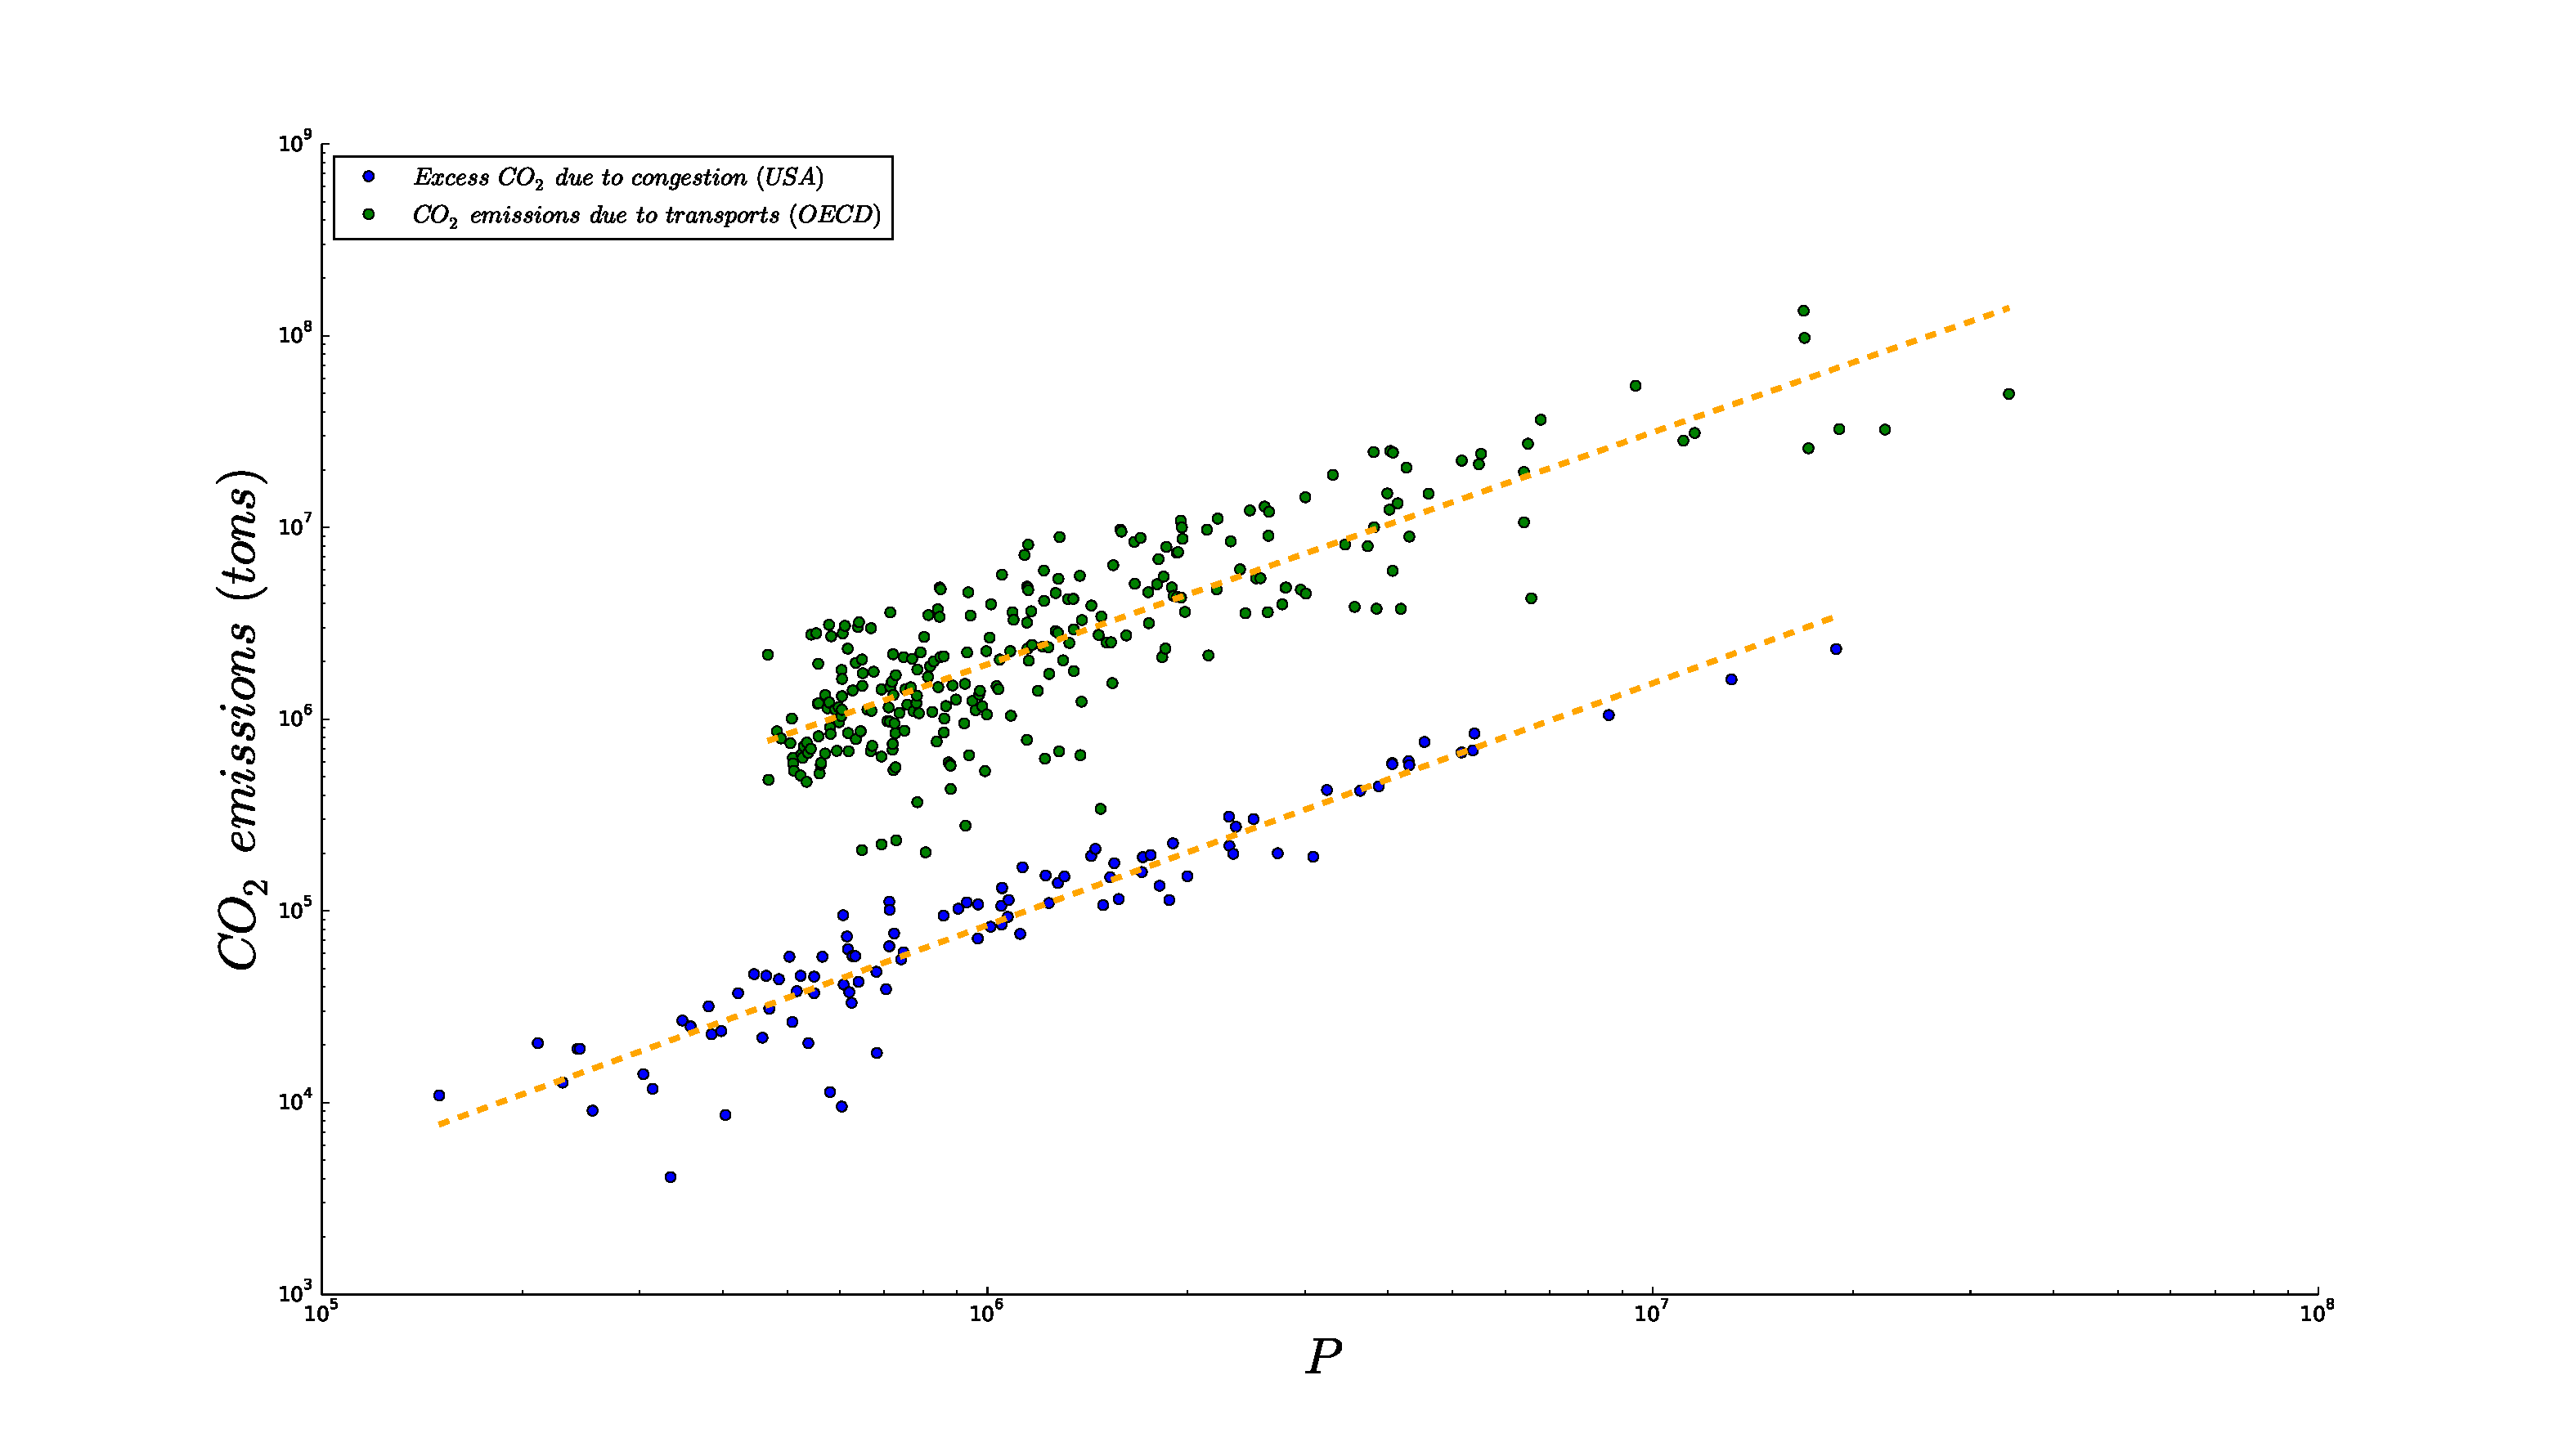
\includegraphics[width=0.9\linewidth]{gfx/chapter-scaling/figure_3.pdf}
\caption{Variation of $CO_2$ emissions due to transport with city size. In blue, excess $CO_2$ (in tons) due to congestion, as given by the Urban Mobility Report (2010) for 101 metropolitan areas in the US~\cite{DataUSA2}. In green, we show the estimated $CO_2$ emissions (in tons) due to transports, as given by the OECD for 268 metropolitan areas in 28 different countries (Data about the total $CO_2$ emissions due to transportation in major metropolitan area in the OECD can be found online~\cite{OECD}). The dashed yellow lines represent the least-square fit assuming a power-law dependency with multiplicative noise, which gives respectively $Q_{CO_2} \sim P^{1.262 \pm 0.089} (r^2=0.94)$ for the US data and $Q_{CO_2} \sim P^{1.212 \pm 0.098} (r^2=0.83)$ for the OECD data.}
\end{figure}

Another important related quantity is the the consumption of gasoline which in principle is proportional to the emission of $CO_2$ and the time spent driving. The total daily gasoline consumption is then given by
%
\begin{equation}
Q_{gas} \sim q\; \ell\; P \left(\frac{P}{c}\right)^{\delta}
\end{equation}
%
where $q$ is the average quantity of gasoline needed per unit time. From this expression, we see that the total daily gasoline consumption per capita scales as
%
\begin{equation}
\frac{Q_{gas}}{P}\sim \ell\, \sqrt{\frac{P}{\rho}} = \ell \sqrt{A}
\end{equation}
%
and is therefore not a simple function of the city density, in contrast with what was suggested by the seminal paper of Newman and Kenworthy~\cite{Newman:1989}. At this stage however, more data about gasoline consumption is needed to test this prediction and draw definitive conclusions.


\section{Discussion}

\subsection{Monocentric versus polycentric}

Although polycentricity emerges naturally from our model as a result of congestion, many circumstances can prevent or foster the appearance of new activity centers in a city. There are many debates as to whether policies should favour polycentric or monocentric developpement of cities. Most of them are based on ideologies and opinions about how cities should be, very few are based on a quantitative understanding of the city as a complex system. Although this only represents a small part of the debate, our model allows to quantify the effect of polycentricity on the total delay due to congestion.

We can indeed compute the total delay due to congestion in the case of a monocentric configuration. In this situation, all the population commutes to a single destination $1$ and we have
%
\begin{equation}
\delta \tau_{mono} = \frac{1}{v}\; \sum_i d_{i1} \left(\frac{P}{c} \right)^\mu = L_{tot} \left(\frac{P}{c} \right)^\mu
\end{equation}
%
It follows, using the expression given above for $L_{tot}$
%
\begin{equation}
\delta\tau_{mono} = \frac{\ell}{v}\; P^{1+\mu}
\end{equation}
%
From the fact that $1+\mu > 1+\frac{\mu}{2\mu+1}$, we indeed find that the total delay due to
congestion is worse for monocentric cities than it is for polycentric cities with the same population, which agrees with the usual intuition. More precisely the ratio of delays is given by
%
\begin{equation}
\frac{\delta\tau_{mono}}{\delta\tau_{poly}}\sim
\left(\frac{P}{c}\right)^{\,\beta}
\end{equation}
%
where the exponent is of order $\beta \approx 0.57\;$. Therefore, even though diseconomies associated with polycentric cities scale superlinearly with population, it would be even worse if we did not let cities evolve from the monocentric case. The same reasoning applies to the consumption of gasoline and the $CO_2$ emissions. This suggests that, everything else being equal, polycentricity should be favoured for quality of life and environmental reasons.
%
\begin{figure}
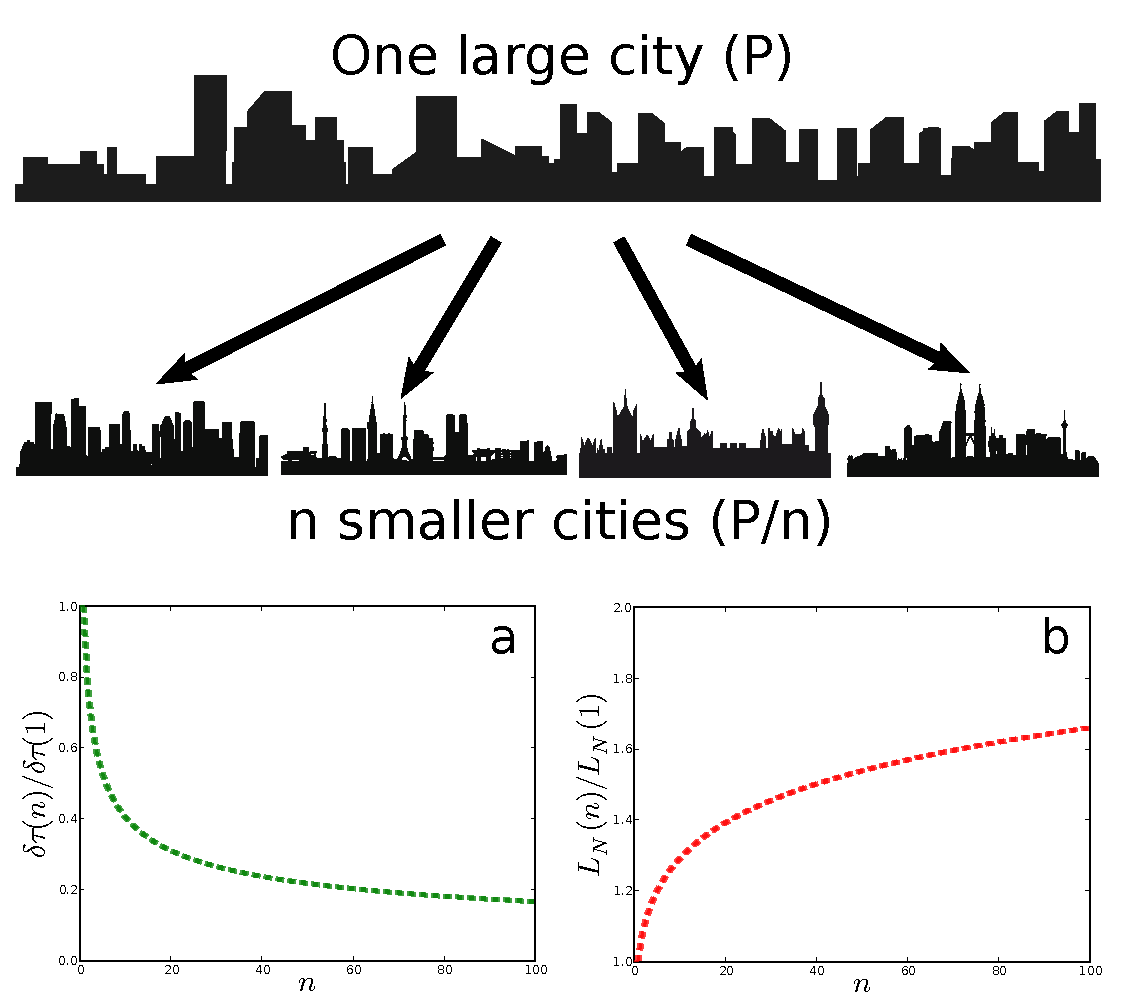
\includegraphics[width=\linewidth]{gfx/chapter-scaling/figure_4.pdf}
\caption{Scaling down. We consider a population $P$ and see how indicators change when we compare it with a system with many cities and the same total population. (a) Variation of the yearly delay per capita due to congestion with the number of cities (normalised by the value $\delta\tau(1)$ corresponding to the single city case). (b) Evolution of the infrastructure length with the number of cities (normalised by the value $L_N(1)$ corresponding to the single city case). Relative gains in terms of commuting time per person decrease faster than infrastructure costs increase, suggesting that life in cities could be improved at a relatively low cost by decentralisation.}
\end{figure}


\subsection{Megapolis versus urban villages} Also, given the superlinear behaviour of the diseconomies associated with living in cities, it is clear that we would be better off living in several smaller cities rather than a single huge city. However, due to the economies of scale realised in large cities, we can wonder whether this is also economically reasonable. If we assume that the total cost of a city of population $P$ is the sum of its infrastructure cost and the economical losses due to congestion we have
%
\begin{equation}
C_T(P) = \epsilon_I \; L_N(P) + \epsilon_C \; \Delta t  \; \delta \tau(P)
\end{equation}
%
where $\epsilon_I$ is the average cost of a kilometer of roads, $\epsilon_C$ the average hourly wage and $\Delta t$ the planning horizon in years (this expression is not exhaustive, as the costs dues to $CO_2$ emissions and gasoline consumptions are not included). The infrastructure needs maintenance, and its cost depends on the planning horizon as well and can be written $\epsilon_I= \epsilon_{B} + \Delta t\; \epsilon_{M}$ where $\epsilon_B$ is the construction cost in $\$/km$ and $\epsilon_M$ the maintenance cost in $ \$/km/year$.

We assume that the population $P$ is distributed among $n$ cities of the same size $P/n$ (see Figure 4). The total lane miles for the $n$ cities reads $L^{(n)}_N(P)=n\,L_N(P/n)$ where $L_N(P)\sim\ell \sqrt{P}\left(\frac{P}{c}\right)^\delta$ is the total lane for one city.  The total congestion delay for $n$ cities is $\delta \tau_n = n\delta\tau(P/n)$ and we thus obtain the total cost $C_T(P,n)$ for $n$ cities
%
\begin{equation}
C_T(P,n) = n^{\, -\delta} \left[ \ell\; \epsilon_I \sqrt{\frac{n}{P}} + \tau\;\epsilon_C \Delta t \right] 
\end{equation}
%
The number of cities $n_{min}$ which minimises the total cost is obtained when $\frac{\mathrm{d} C}{\mathrm{d} n} = 0$, leading to (for $\Delta t\gg 1$)
%
\begin{equation}
n_{min} = P \left[ \left( \frac{2\delta}{1+\delta} \right) \frac{\epsilon_C}{\epsilon_M} \frac{\tau}{\ell} \right]^2
\end{equation}
%
(the actual number of cities is of course an integer, and can be taken as the nearest integer from $n_{min}$ for instance).  It is then economically advantageous to divide the population in several cities if $n_{min} > 2$. To illustrate this point, we compute the number of cities which would minimise the cost for a world population $P \approx 10^9$. The World Bank estimates the maintenance cost of roads to be of the order of $\epsilon_M \approx 10^5\; \$/km/year$, and the average hourly wage to be of the order of $\epsilon_C \approx 10\; \$/h$, the value of $\delta$ is taken from the measures on US data, $\delta \approx 0.27$, and $\tau / \ell \approx 10\; km/h$. We then obtain
%
\begin{equation}
n_{min} \approx 180
\end{equation}
%
which gives an average city size of $P/n\approx 5,500,000$. This result is to put in perspective with the fact that the world hosts
$40$ or so cities with over $5,500,000$ inhabitants and that this number is still increasing. 

\subsection{The most economical population distribution}

The previous results assume that we split a large city into many cities of the same size. The cities are however organized in various sizes distributed according to something that can be approximated by a Pareto distribution, as known since Zipf's work~\cite{Zipf:1949}. It is still unclear why we observe such a convergence~\cite{Batty:2006,Cristelli:2012}. We propose here a new perspective to this debate by asking: Assuming cities are distributed according to a Pareto distribution, what value of the exponent minimises the overall cost? Indeed from above the total cost for a population size $x$ is given at large times by
%
\begin{equation}
C_T(x) = \epsilon_M\Delta t \; L_N(x) + \epsilon_C \; \Delta t  \; \delta \tau(x)
\end{equation}
%
We assume that the population is distributed according to 
%
\begin{equation}
\mathcal{P}(x)=(\gamma-1) x^{-\gamma}\;\;\;\text{for}\;\;x\in[1,\Lambda ]
\end{equation}
%
with $\gamma>1$ and a cut-off population $\Lambda \gg 1$ (which is at most equal to the world's population). The average cost is then given by
%
\begin{equation}
\overline{C_T} = \int_1^\Lambda \mathcal{P}(x)\,C_T(x)\,dx
\end{equation}
%
leading to
%
\begin{equation}
\overline{C_T} = \frac{\Delta t\, \ell}{c^\delta}\,\left(\gamma - 1 \right) \left[ \epsilon_M\frac{\Lambda^{-\gamma+\delta+\frac{3}{2}}-1}{-\gamma+\delta+\frac{3}{2}} + \frac{\epsilon_C}{v}\frac{\Lambda^{-\gamma+\delta+2}-1}{-\gamma+\delta+2} \right]
\end{equation}
%
The only consistent solution is obtained for $\gamma < \delta + 2$. The dominant term for $\Lambda \gg 1$ is given by
%
\begin{equation}
\overline{C_T}\simeq \frac{\Delta t\,\epsilon_C\, \ell}{c^\delta}\,\left(\gamma - 1 \right) \left[ \frac{\Lambda^{-\gamma+\delta+2}}{-\gamma+\delta+2} \right]
\end{equation}
%
The optimal power law distribution minimizes the average cost and is such that $\frac{{\rm d} \overline{C_T}}{{\rm d} \gamma} = 0$. We obtain the following equation
%
\begin{equation}
\frac{1+\delta}{\delta+2-\gamma} = \left(\gamma - 1\right) \ln \Lambda
\end{equation}
%
and in the limit $\Lambda \gg 1$ we obtain the optimal value for $\gamma$
%
\begin{equation}
\gamma^* = 2+\delta - \frac{1}{\ln \Lambda}
\end{equation}
%
Numerically, $\delta \approx 0.32$ and $\Lambda \approx 10^{9}$, leading to $\gamma^* \approx 2.27$. It is interesting to note that this value would lead to a rank-plot exponent ($\approx 0.78$) not far from those measured on different countries around the world~\cite{Soo:2005}. Although we do not pretend that the above reasoning provides a definitive answer to the Zipf puzzle, it nevertheless suggests that the broad diversity of population might derive from economical considerations, and that there may be a connection between the Zipf law exponent and optimality considerations.


\subsection{Outlook}

The superlinear increase of congestion delay with population, and thereby of gasoline consumption and of $CO_2$ emissions, has terrible consequences on the economy, the environment, health and well-being. The outlook is nothing short of grim in our ever-urbanising world. As the proportion of human beings living in cities dramatically increases --the UN expects the world population to be $67\%$ urban in 2050~\cite{UN:2011}-- wages are likely to increase~\cite{Bettencourt:2007} but not enough to compensate for the negative effects of congestion. As a result, if the individual car stays the dominant transportation mode, cities will put more strain on people's life, while acting as catalysts for the production of $CO_2$ greenhouse gas, responsible for an overall increase of the planet's temperature~\cite{Oreskes:2004}. It is currently believed that advantages associated with living in a large city outweigh the costs. Our results reveal however the existence of very rapidly growing problems such as congestion and $CO_2$ emissions, which inevitably begs the question of the sustainability of large cities. It might be time to cut down considerably the use of individual vehicles, or to consider the possibility of living in smaller or medium sized cities: the infrastructure costs ($L_N$) may be larger, but the impact on the environment ($CO_2$ emissions) and on the well-being of people (delays in congestion) would be beneficial (see Figure 3).

The most striking fact about the above results is that despite the apparence of complexity that is conveyed by cities, most of their structure can be explained by the very simple and universal desire for the best achievable balance between income and commuting costs. Our model unifies mobility patterns, spatial structure of cities and allometric scalings in a framework that can be built upon. More work is needed in order to integrate information about firm locations, the influence of public transportation on mobility patterns~\cite{Roth:2011}, the effect of the integration of cities into urban systems~\cite{Rozenblat:2007}, to understand the fluctuations around the average trends, and to test the validity of the model on different sets of data. We believe however that the results presented here represent a crucial step towards a scientific understanding of cities.


\section{What cities?}
\label{sec:what_cities_}

\cite{Louf:2014_smog} for problem with the $CO_2$\\
\cite{Arcaute:2015} for variation of exponents with city definition.


The success of natural sciences lies in their great emphasis on the role of quantifiable data and their interplay with models. Data and models are both necessary for the progress of our understanding: data generate stylized facts and put constraints on models. Models on the other hand are essential to comprehend the processes at play and how the system works. If either is missing, our understanding and explanation of a phenomenon are questionable. This
issue is very general, and affects all scientific domains, including the study of cities. \\

Until recently, the field of urban economics essentially consisted in untested laws and theories, unjustified concepts that supersede empirical evidence~\cite{Bouchaud:2008}. Without empirical validation, it is not clear what these models teach us about cities. The tide has turned in recent years, however: the availability of data is increasing in size and specificity, which has led to the discovery of new stylized facts and opened the door to a new science of cities~\cite{Batty:2013}. The recent craze for scaling laws~\cite{Batty:2008,Bettencourt:2007,Pumain:2004}, for instance, has been an important new step in the study of urban systems.

These laws present themselves as a power-law relationship between socioeconomic (GDP, number of patents), structural (length of roads, of cables) quantities $Y$, and the size of the population $P$ of the city:

\begin{equation}
Y = P^{\, \beta}
\end{equation}


where the exponent $\beta$ can be different from $1$. This type of scaling relation is a signature
of various processes governing the phenomenon under study, especially when the exponent
$\beta$ is not what is naively expected~\cite{Barenblatt:2003}. However, as more and more scaling
relationships are being reported in the literature, it becomes less and less clear what we really
learn from these empirical findings. Mechanistic insights about these scalings are usually
nonexistent, often leading to misguided interpretations.\\

\begin{figure}[!h]
	\centering
	%\includegraphics[width=0.49\textwidth]{figure.pdf}
	\caption{ {\bf Are larger cities greener or smoggier?} Scaling of transport-related $CO_2$
emissions with the population size for US cities from the same dataset but at different aggregation
levels. In red, the aggregation is done at the level of urban areas and in green for combined statistical
areas. Depending on the definition of the city, the scaling exponents are qualitatively different, leading
to two opposite conclusions. Data on $CO_2$ emissions were obtained from the Vulcan Project (\url{http://
vulcan.project.asu.ed}) (see~\cite{Fragkias:2013,Oliveira:2014}). Data on the population of urban areas and
metropolitan statistical areas were obtained from the Census Bureau (\protect\url{http://www.census.org}). \label{fig}}
\end{figure}


A striking example of the fallacies which hinder the interpretation and application
of scaling is given by different studies on $CO_2$ emissions due to transportation~\cite{Fragkias:2013,Glaeser:2010,Oliveira:2014,Rybski:2013}. The topic
is particularly timely: pollution peaks occur in large cities worldwide with a seemingly
increasing frequency, and are suspected to be the source of serious health problems~\cite{Bernstein:2004}. Glaeser and Kahn~\cite{Glaeser:2010}, Rybski et al~\cite{Rybski:2013}, Fragkias et al~\cite{Fragkias:2013}, and Oliveira et al~\cite{Oliveira:2014} are interested in how $CO_2$ emissions scale with the population size
of cities. The question they ask is simple: Are larger cities greener---in the sense that there
are fewer emissions per capita for larger cities---or smoggier? Surprisingly, these different
studies reach contradictory conclusions. We identify here two main sources of error which
originate in the lack of understanding of the mechanisms governing the phenomenon.

The first error concerns the estimation of the quantity $Q_{CO_2}$ of $CO_2$ emissions due to
transportation. In the absence of direct measures, Glaeser and Kahn~\cite{Glaeser:2010} have chosen
to use estimations of $Q_{CO_2}$ based on the total distance traveled by commuters. This is in fact
incorrect, and in heavily congested urban areas the relevant quantity is the total time spent
in traffic~\cite{Louf:2013}. Using distance leads to a serious underestimation of
$CO_2$ emissions: the effects of congestion are indeed strongly nonlinear, and the time spent
in traffic jams is not proportional to the traveled distance. As a matter of fact, commuting
distance and time scale differently with population size, and the time spent commuting and
$CO_2$ emissions scale with the same exponent~\cite{Louf:2014}.

The second, subtler, issue lies in the definition of the city itself, and over which
geographical area the quantities $Q_{CO_2}$ and $P$ should be aggregated. There is currently great
confusion in the literature about how cities should be defined, and scientists, let alone the
various statistical agencies in the world, have not yet reached a consensus. This is a crucial
issue as scaling exponents are very sensitive to the definition of the city~\cite{Arcaute:2013}. $CO_2$ emissions are no exception: aggregating over urban areas or metropolitan
statistical areas entails radically different behaviours (see figure~\ref{fig}). For the US, using the
definition of urban areas provided by the Census Bureau (\url{http://www.census.org}), one finds
that $CO_2$ emissions per capita sharply increase with population size, implying that larger
cities are less green. Using the definition of metropolitan statistical areas, also provided by
the Census Bureau, one finds that $CO_2$ emissions per capita decrease slightly with population
size, implying that larger cities are greener.\\



Faced with these two opposite results, what should one conclude? Our point is that, in
the absence of a convincing model that accounts for these differences and how they arise,
nothing. Scaling relationships, and more generally data analysis, have an important role
to play in the rising new science of cities. But, as the previous discussion illustrates, it is
dangerous to interpret empirical results without any mechanistic insight. Conclusions cannot
safely be drawn from data analysis alone.

From a policy point of view, now, what should one do to curb CO2 emissions? Favour
the growth of large urban areas or the repartition of population in less populated cities?
Both can be argued by considering data analysis alone. It should therefore be obvious that,
until they have a satisfactory understanding of the mechanisms responsible for the observed
behaviours, scientists should refrain from giving policy advice that might have unforeseen,
disastrous consequences. If they choose to do so anyway, policy makers should be wary
about what is, at best, a shot in the dark

\section{Poviso}
\label{sec:poviso}

Scaling laws are useful tool to probe the system city, but they are not
everything. They provide an extraordinarily easy way to explore the properties
of urban systems: the amount of data required is minimal, the treatment
trivial. However, while it may be useful to declutter the investigation field
and help clear a couple of paths, and help establish a large-scale understanding
of the system, this is done at the expense of an extensive coverage of the
underlying phenomena. Scalings can be seen as a gateway to the study of cities,
but they cannot be the study itself.

 % Chapter 2

%------------------------------------------------

\ctparttext{Segregation is a notion that is difficult to define, hence the
extensive literature concerning segregation in the literature. In this part, we
propose to measure segregation as a deviation to the unsegregated city. We thus
provide a strong theoretical basis for the location coefficient. We further
derive a measure of attraction of the different categories, that allows us to
define unambiguously classes for the original categories. We study the
properties of neighbourhoods of different classes. We revisit the poor
center/rich suburb distinction. Finally, we propose a new measure of segregation
that takes space into account.} % Text on the Part 2 page describing the content in Part 2

\part{Socio-spatial stratification} % Second part of the thesis

% !TEX root = ../thesis-example.tex
%
\chapter{The socio-spatial stratification in cities}
\label{sec:concepts}


\begin{flushright}{\slshape    
The limits of my language\\
Are the limits of my world.} \\ \medskip
--- Ludwig Wittgenstein 
\end{flushright}

\section{Introduction}
\label{sec:introduction}

\section{Null model: the unsegregated city}
\label{sec:null_model_the_unsegregated_city}

\section{Measuring the attraction and repulsion of categories}
\label{sec:measuring_the_attraction_and_repulsion_of_categories}

\section{The emergent social classes}
\label{sec:the_emergent_social_classes}

\section{Clustering and concentration}
\label{sec:clustering_and_concentration}

\section{Poor centers, rich suburbs?}
\label{sec:poor_centers_rich_suburbs_}

\section{A new measure of segregation}
\label{sec:a_new_measure_of_segregation}
 % Chapter 2

%------------------------------------------------

\ctparttext{Cities and systems of cities are irrigated in people, energy,
information and goods thanks to various spatial networks. In this part, we show
how a new perspective on street patterns, and the use of OpenStreetMaps'
database allow us to provide a classification of cities based on their street
pattern. We then propose a large-scale description of subway and railway
networks, and are able to predict many of their properties based on the
properties of the underlying city or country.} % Text on the Part 2 page describing the content in Part 2

\part{Urban Networks} % Second part of the thesis

\include{chapters/chapter-networks} % Chapter 2


%------------------------------------------------

\ctparttext{Cities are not closed systems. Neither do they evolve in isolation.
Rather, they interact in what has been called a system of cities. In this part,
we focus on the movements of populations inside a system of city. We sutyd the
network of residential migrations in the US, describe some of its properties,
and show some unexpected consequences. Last, but not least, we show how Zipf's
law finds a natural explanation in when considering the motion of people.} % Text on the Part 2 page describing the content in Part 2

\part{Systems of cities} % Second part of the thesis

% !TEX root = ../thesis-example.tex
%
\chapter{The metropolitan blend}
\label{chap:metropolitan_blend}

\begin{flushright}{\slshape
You cannot base a general mathematical theory\\
on imprecisely defined concepts.\\
You can make some progress that way; \\
but sooner or later the theory is bound to dissolve in ambiguities\\ 
which prevent you from extending it further.} \medskip
--- E.T. Jaynesi~\cite{Jaynes:1986}
\end{flushright}
 % The metropolitan blend 
% !TEX root = ../thesis-example.tex
%
\chapter{Zipf's law and derivatives}
\label{chap:zipf_law}

 % Some work on Zipf
% !TEX root = ../thesis-example.tex
%
\chapter{The mystery of urban hierarchy}
\label{sec:concepts}

\begin{flushright}{\slshape    
The usual complaint about economic theory is that our models are
oversimplified---that offer excessively neat views of complex, messy reality.
[..] In one important case, the reverse is true: we have complex, messy models,
yet reality is startingly neat and simple.
} \\ \medskip
--- Paul Krugman~\cite{Krugman:1996}
\end{flushright}

\section{Introduction}
\label{sec:introduction}

\cite{Krugman:1996}
\cite{Gabaix:1999}
\cite{Batty:2013} for issues with Gibrat.
\cite{Cristelli:2012}
\cite{Batty:2006}

\section{The model}
\label{sec:the_model}


We write that 

\begin{equation}
    \partial_t P = \left(1-b-d\right)\,P + M_i^U + M_i^E
\end{equation} 

If the population is increasing wuch that

\begin{equation}
    P_{t+1} = \gamma_t\,P_t + \epsilon_t
\end{equation}

where $\epsilon_t$ is a small random increment with
$\mathrm{E}\left[\epsilon_t]\right] = \overline{\epsilon} > 0$. Whatever the
initial distirbution, the city-size distribution converges to a power-law with
and exponent $\zeta$ such that $\mathrm{E}\left[\gamma^\zeta\right] = 1$ (cite
Sornette). For small values of $\overline{\epsilon}$ we have

\begin{equation}
    \zeta = 1 + O(\epsilon)
\end{equation}

If the random variable is log-normally distributed, we have

\begin{equation}
    \zeta = 1 - \frac{2}{\sigma^2} \ln\left(1 -
    \frac{\overline{\epsilon}}{\overline{P}}\right)
\end{equation}

where $\overline{P}$ is the average size of a city. Therefore, the Zipf exponent
reads

\begin{equation}
    \boxed{    \alpha = \frac{1}{1 - \frac{2}{\sigma^2} \ln\left(1 -
\frac{\overline{\epsilon}}{\overline{P}}\right)}}
\end{equation}

From this equation one can clearly see that $\alpha > 1$ if and only if
$\overline{\epsilon} < 0$, that is when there is on average an outward flow
towards the outside of the system of cities (rural areas). On the other hand, we
have $\alpha < 1$ when $\overline{\epsilon} < 1$, that is when an important
rural exodus is happening, and $\alpha = 1$ if and only if $\overline{\epsilon}
= 0$, that is when the system of cities is at equilibrium with the rural
environment.
 % A model to explain Zipf's law

%------------------------------------------------

\ctparttext{In this part we summarize the results obtained in this thesis and
outline some possible future axes of research.} % Text on the Part 2 page describing the content in Part 2

\part{Conclusion} % Second part of the thesis

% !TEX root = ../thesis-example.tex
%
\chapter{Conclusion}
\label{sec:conclusion}

\begin{flushright}{\slshape    
If people never did silly things\\
nothing intelligent would ever get done.} \\ \medskip
--- Ludwig Wittgenstein 
\end{flushright}


\section{What the past 3 years have brought}
\label{sec:what_the_past_3_years_have_brought}


What I find striking is the propention of the different communities to ignore
one another. Although there is a lot to say about physicists being ignorant of
most of the literature in social sciences, there is also a lot to say about
social sciences applying tools as black boxes, without any reflexion on the
meaning of the formula that is being applied. Despite an important literature on
the topic, we can still see exponents of power-law distribution estimated using
the Least-Squares method. A lot of the litterature on complex network is also
applied carelessly, a big victim being the algorithms of community detection (no
reflection on the meaning of communities, for instance). It is a real shame,
because we need people with quantitative skills to manipulate formulas and
create new measures, but we also need qualitative skills to manipulate concept
and interpret the significance of the results. While we cannot expect a
physicist or a computer scientitist to know all the literature in a field that
is not his own, we cannot expect social scientists to have strong quantitative
skills. The real solution resides in the collaboration.\\

It is ignorance, not knowledge, that fuels science.

\section{The thesis I wish I wrote}
\label{sec:limitations}

The temptation is great, looking back on $3$ years of work with a more
experienced eye, to understate the contributions of this thesis and their
potential applications. The thesis that you have been reading is of course very
different from the thesis I would have liked to write. Frustrating realisation
that good research takes time. It takes time for the literature to sink in, it
takes time to understand the limits of your contribution, it takes time to get
at the bottom of a field. Not that I would do anything differently---I
couldn't--- but I now start to realise the work that is yet to be accomplished.
And that is only for what I am aware should be done, new problems and questions
are ready to pop out of nowhere at any time.\\

So what would have I write about---or at least try to---if I had to start my
thesis all over again? This is another way of saying: what are the next steps?
How does the research presented here fit in this picture?\\

I would start being more careful with the concepts that are being used. Starting
with the basics, with the single noun that was most often printed in these
pages: Cities. Despite it being our object study, it seems that the very
definition of this object is something obscure, somewhat hidden in the
literature. At least, it is something that is not really talked about in the
literature. Yet, if we want to exhibit robust empirical results, we need to
start worrying about the definition of the system we are studying. We need to
know \emph{what} cities we are talking about.\\


Once the boundaries are defined, we can start studying the way objects are
scattered within them. By objects, I mean buildings, roads, and first and
foremost people. The way we traditionally study the repartition of objects in
space is through the study of densities. An interesting thing to study would for
instance be the population density profile, possibly at different times of the
day. But density profiles are too complicated to comprehend for our brains,
especially when cities get large. Spatial statistics attemps to solve this
problem by providing simple measures, that extract a single number from
distributions. A single number is however too simple to be able to describe
accurately complex density profiles. What we need is a meso-scale
representation, somewhere between the micro-scale picture (the density profile
itself) and the macro-scale picture (a single number to summarize the density
profile). A requirement for this method is to make the definition of centers (or
hotspots) natural, because centers are a meso-scale representation of density
profiles already. This should make the notion of a center defined from first
principle, which would then allow to discuss the \emph{absolute} number of
centers in the city. Until now, because we do not clearly understand what the
meaning of the centers we obtain with the different existing methods, we are
only able to get numbers that are useful for inter-urban comparisons. The
spatial contiguity is not even taken into account!  This is where the model on
the polycentric transition of cities, presented in
Chapter~\ref{chap_monocentric} fits. Although I do not expect the scaling of the
number of centers with city size to change (but who knows), having a more
accurate description of the poly- or monocentric structure of population
distributions at different times of the day should help put more constrains on
existing models, and give hints for improvement of the existing models.\\


Once one is able to provide an accurate description of densit profiles, the
possibilities start to diverge. An obvious worry, when one has a picture of the
city's population at different times of the day, is the way these profile
transform one into another. This is linked to commuting---but not only,
commuting representing only $20\%$ of total travels in the
US~\cite{FHWA-PL-11-022}--- and the study of congestion of networks. We can
first wonder the link between the urban form (typically the residential and
employment densities) and mobility patterns. This is tackled in the excess
commuting literature (a few references here). There fit both the first and
second part of this thesis.\\ A futher worry linked to commuting is that of
congestion: understanding how congestion are formed, how they propagate and
devise strategies to mitigate them, either by influencing the transportation
infrastructure, the spatial repartition of residences and employment, or the
behaviour of people themselves.  This is far from being a recent worry, and
there already is an impressively vast literature on the topic [cite review].
Yet, there is room for new approaches that leverage the knowledge we have about
network and phase transition in physics. A first step in this direction has been
made by the authors of~\cite{Daqing:2015}, but there is surely more to be
understood and discovered.  Modeling congestion also implies understanding the
individual behaviour of people when they are moving from a point to another in
cities. Altough most research nowadays assume that people choose the shortest
(time or distance) path, GPS data now provide overwhelming evidence that this is
not the case [Manley, etc]. So, while there is a clear need to understand the
meso-scopic picture (how congestion spread), there is also is a critical need to
understand the microscopic picture (how people behave).\\

So far we have talked about the movement induced by the spatial mismatch between
residential areas and activity areas. One might also want to study the
characteristics of the spatial repartition of people. Inhabitants of cities are
not just a combination of a latitude and a longitude, a point on a map. Like you
and me, they are characterised by different qualities, some of which are
measurable: say their income, their education level, their ethnicity, etc. A
natural question, that has interested sociologist and geographers, is to wonder
whether people's residence is independent of these characteristics, or whether
these characteristics have an influence on the spatial repartition of
individuals. In other words, the study of residential segregation. A
contribution of this thesis is to provide a rigorous method to study the
patterns of segregation in the presence of multiple categories, and to identify
`neighbourhoods', that is regions in the city where individual belonging to a
particular category. I hope that, along with the improvement of the
characterisation of density profiles, we will be able to describe more
accurately the spatial patterns of segregation, which should hopefully lead to a
better understanding of this phenomenon, and better models.\\

The list is still long, and gets more and more speculative as we deviate from
the questions that are directly entailed by the work I have presented here.


\section{Future work}
\label{sec:future_work}

I do believe there is a cruel lack of serious empirical work in the field. This
should be quickly solved, thanks to the information technologies that are now
available. But there is a bigger problem looming over our heads. The
uncomfortable fact that our fundamental object, the city, is an ill-defined
object. And that most empirical studies possibly rely on definitions of a city
that are not suited to the study they undertake. 
This lack of serious definition compromises the comparison between cities of
different countries (as I saw in the fingerprint paper), or different points in
time. I am, of course, not the first person to acknowledge this empirical
difficulty. In fact, it has been a long-time worry of geographers who have been
trying to produce harmonised database for a long time (cite
Bretagnolle, Pumain, any reference on harmonised database). Yet, we still lack
of an unambiguous, theoretically grounded definition of what a city is. And this
is problematic, since statistical institutes' results are based on what is
believed to be the best definition of the city at a time, which influences the
results, etc.
The problem is that it is unlikely there is only one way to define the object
city, but rather different definitions that depend on what we are studying.
People are usually confused by the existence of different definitions.


 % Chapter 2


%----------------------------------------------------------------------------------------
%	THESIS CONTENT - APPENDICES
%----------------------------------------------------------------------------------------

%\appendix

%\part{Appendix} % New part of the thesis for the appendix

%\include{Chapters/Chapter0A} % Appendix A
%\include{Chapters/Chapter0B} % Appendix B - empty template

%----------------------------------------------------------------------------------------
%	POST-CONTENT THESIS PAGES
%----------------------------------------------------------------------------------------

\cleardoublepage% Bibliography

\label{app:bibliography} % Reference the bibliography elsewhere with \autoref{app:bibliography}

\manualmark
\markboth{\spacedlowsmallcaps{\bibname}}{\spacedlowsmallcaps{\bibname}} 
\refstepcounter{dummy}

\addtocontents{toc}{\protect\vspace{\beforebibskip}} % Place the bibliography slightly below the rest of the document content in the table of contents
\addcontentsline{toc}{chapter}{\tocEntry{\bibname}}

\bibliographystyle{plainnat}

\bibliography{Bibliography} % Bibliography
\cleardoublepage% Colophon (a brief description of publication or production notes relevant to the edition)

\pagestyle{empty}

\hfill

\vfill

\pdfbookmark[0]{Colophon}{colophon}

\section*{Colophon}

This document was typeset using the typographical look-and-feel \texttt{classicthesis} developed by Andr\'e Miede. The style was inspired by Robert Bringhurst's seminal book on typography ``\emph{The Elements of Typographic Style}''. \texttt{classicthesis} is available for both \LaTeX\ and \mLyX: 

\begin{center}
\url{http://code.google.com/p/classicthesis/}
\end{center}

\noindent Happy users of \texttt{classicthesis} usually send a real postcard to the author, a collection of postcards received so far is featured here: 

\begin{center}
\url{http://postcards.miede.de/}
\end{center}
 
\bigskip

\noindent\finalVersionString % Colophon
\cleardoublepage% Declaration

\refstepcounter{dummy}
\pdfbookmark[0]{Declaration}{declaration} % Bookmark name visible in a PDF viewer

\chapter*{Declaration} % Declaration section text

\thispagestyle{empty}

Put your declaration here.
\bigskip
 
\noindent\textit{\myLocation, \myTime}

\smallskip

\begin{flushright}
\begin{tabular}{m{5cm}}
\\ \hline
\centering\myName, \today \\
\end{tabular}
\end{flushright}
 % Declaration

%----------------------------------------------------------------------------------------

\end{document}
